\documentclass[10pt]{article}
\usepackage[utf8]{inputenc}
\usepackage[T1]{fontenc}
\usepackage{amsmath}
\usepackage{amsfonts}
\usepackage{amssymb}
\usepackage[version=4]{mhchem}
\usepackage{stmaryrd}
\usepackage{bbold}
\usepackage{graphicx}
\usepackage[export]{adjustbox}
\graphicspath{ {./images/} }
\usepackage{mathrsfs}

\title{Chapter 29 }

\author{}
\date{}


\begin{document}
\maketitle
\section{Machine Learning}
\subsection{Introduction}
This chapter reviews machine learning methods for econometrics. This is a large and growing topic so our treatment is selective. This chapter briefly covers ridge regression, Lasso, elastic net, regression trees, bagging, random forests, ensembling, Lasso IV, double-selection/post-regularization, and double/debiased machine learning.

A classic reference is Hastie, Tibshirani, and Friedman (2008). Introductory textbooks include James, Witten, Hastie, and Tibshirani (2013) and Efron and Hastie (2017). For a theoretical treatment see Bühlmann and van der Geer (2011). For reviews of machine learning in econometrics see Belloni, Chernozhukov and Hansen (2014a), Mullainathan and Spiess (2017), Athey and Imbens (2019), and Belloni, Chernozhukov, Chetverikov, Hansen, and Kato (2021).

\subsection{Big Data, High Dimensionality, and Machine Learning}
Three inter-related concepts are "big data", "high dimensionality", and "machine learning".

Big data is typically used to describe datasets which are unusually large and/or complex relative to traditional applications. The definition of "large" varies across discipline and time, but typically refers to datasets with millions of observations. These datasets can arise in economics from household census data, government administrative records, and supermarket scanner data. Some challenges associated with big data are storage, transmission, and computation.

High Dimensional is typically used to describe datasets with an unusually large number of variables. Again the definition of "large" varies across applications, but typically refers to hundreds or thousands of variables. In the theoretical literature "high dimensionality" is used specifically for the context where $p>n$, meaning that the number of variables $p$ greatly exceeds the number of observations $n$.

Machine Learning is typically used to describe a set of algorithmic approaches to statistical learning. The methods are primarily focused on point prediction in settings with unknown structure. Machine learning methods generally allow for large sample sizes, large number of variables, and unknown structural form. The early literature was algorithmic with no associated statistical theory. This was followed by a statistical literature examining the properties of machine learning methods, mostly providing convergence rates under sparsity assumptions. Only recently has the literature expanded to include inference.

Machine learning embraces a large and diverse set of tools for a variety of settings, including supervised learning (prediction rules for $Y$ given high-dimensional $X$ ), unsupervised learning (uncovering structure amongst high-dimensional $X$ ), and classification (discrete choice analysis with highdimensional predictors). In this chapter we focus on supervised learning as it is a natural extension of linear regression.

Machine learning arose from the computer science literature and thereby adopted a distinct set of labels to describe familar concepts. For example, it speaks of "training" rather than "estimation" and "features" rather than "regressors". In this chapter, however, we will use standard econometric language and terminology.

For econometrics, machine learning can be thought of as "highly nonparametric". Suppose we are interested in estimating the conditional mean $m(X)=\mathbb{E}[Y \mid X]$ when the shape of $m(x)$ is unknown. A nonparametric analysis typically assumes that $X$ is low-dimensional. In contrast, a machine learning analysis may allow for hundreds or even thousands of regressors in $X$, and does not require prior information about which regressors are most relevant.

Connections between nonparametric estimation, model selection, and machine learning methods arise in tuning parameter selection by cross-validation and evaluation by out-of-sample prediction accuracy. These issues are taken seriously in machine learning applications; frequently with multiple levels of hold-out samples.

\subsection{High Dimensional Regression}
We are familiar with the linear regression model $Y=X^{\prime} \beta+e$ where $X$ and $\beta$ are $p \times 1$ vectors ${ }^{1}$. In conventional regression models we are accustomed to thinking of the number of variables $p$ as small relative to the sample size $n$. Traditional parametric asymptotic theory assumes that $p$ is fixed as $n \rightarrow \infty$ which is typically interpreted as implying that $p$ is much smaller than $n$. Nonparametric regression theory assumes that $p \rightarrow \infty$ but at a much slower rate than $n$. This is interpreted as $p$ being moderately large but still much smaller than $n$. High-dimensional regression is used to describe the context where $p$ is very large, including the case where $p$ is larger than $n$. It even includes the case where $p$ is exponentially larger than $n$.

It may seem shocking to contemplate an application with more regressors than observations. But the situation arises in a number of contexts. First, in our discussion of series regression (Chapter 20) we described how a regression function can be approximated by an infinite series expansion in basis transformations of the underlying regressors. Expressed as a linear model this implies a regression model with an infinite number of regressors. Practical models (as discussed in that chapter) use a moderate number of regressors in estimated regressions because this provides a balance between bias and variance. This latter models, however, are not the true conditional mean (which has an infinite number of regressors) but rather a low-dimensional best linear approximation. Second, many economic applications involve a large number of binary, discrete, and categorical variables. A saturated regression model converts all discrete and categorical variables into binary variables and includes all interactions. Such manipulations can result in thousands of regressors. For example, ten binary variables fully interacted yields 1024 regressors. Twenty binary variables fully interacted yields over one million regressors. Third, many contemporary "big" datasets contain thousands of potential regressors. Many of the variables may be low-information but it is difficult to know a priori which are relevant and which irrelevant.

When $p>n$ the least squares estimator $\widehat{\beta}_{\text {ols }}$ is not uniquely defined because $\boldsymbol{X}^{\prime} \boldsymbol{X}$ has deficient rank. Furthermore, for $p<n$ but "large" the matrix $\boldsymbol{X}^{\prime} \boldsymbol{X}$ can be near-singular or ill-conditioned so the least squares estimator can be numerically unstable and high variance. Consequently we turn to estimation methods other than least squares. In this chapter we discuss several alternative estimation methods, including ridge regression, Lasso, elastic net, regression trees, and random forests.

${ }^{1}$ In most of this textbook we have denoted the dimension of $X$ as $k$. In this chapter we will instead denote the dimension of $X$ as $p$ as this is the custom in the machine learning literature.

\section{$29.4$ p-norms}
For discussion of ridge and Lasso regression we will be making extensive use of the 1-norm and 2norm, so it is useful to review the definition of the general p-norm. For a vector $a=\left(a_{1}, \ldots, a_{k}\right)^{\prime}$ the p-norm $(p \geq 1)$ is

$$
\|a\|_{p}=\left(\sum_{j=1}^{k}\left|a_{j}\right|^{p}\right)^{1 / p} .
$$

Important special cases include the 1-norm

$$
\|a\|_{1}=\sum_{j=1}^{k}\left|a_{j}\right|
$$

the 2-norm

$$
\|a\|_{2}=\left(\sum_{j=1}^{k} a_{j}^{2}\right)^{1 / 2},
$$

and the sup-norm

$$
\|a\|_{\infty}=\max _{1 \leq j \leq k}\left|a_{j}\right| .
$$

We also define the "0-norm"

$$
\|a\|_{0}=\sum_{j=1}^{k} \mathbb{1}\left\{a_{j} \neq 0\right\},
$$

the number of non-zero elements. This is only heuristically labeled as a "norm".

The p-norm satisfies the following additivity property. If $a=\left(a_{0}, a_{1}\right)$ then

$$
\|a\|_{p}^{p}=\left\|a_{0}\right\|_{p}^{p}+\left\|a_{1}\right\|_{p}^{p} .
$$

The following inequalities are useful. The Hölder inequality for $1 / p+1 / q=1$ is

$$
\left|a^{\prime} b\right| \leq\|a\|_{p}\|b\|_{q} .
$$

The case $p=1$ and $q=\infty$ is

$$
\left|a^{\prime} b\right| \leq\|a\|_{1}\|b\|_{\infty} .
$$

The Minkowski inequality for $p \geq 1$ is

$$
\|a+b\|_{p} \leq\|a\|_{p}+\|b\|_{p} .
$$

The p-norms for $p \geq 1$ satisfy norm monotonicity. In particular

$$
\|a\|_{1} \geq\|a\|_{2} \geq\|a\|_{\infty} .
$$

Applying Hölder's (29.1) we also have the inequality

$$
\|a\|_{1}=\sum_{j=1}^{k}\left|a_{j}\right| \mathbb{1}\left\{a_{j} \neq 0\right\} \leq\|a\|_{2}\|a\|_{0}^{1 / 2} .
$$

\subsection{Ridge Regression}
Ridge regression is a shrinkage-type estimator with similar but distinct properties from the JamesStein estimator (see Section 28.20). There are two competing motivations for ridge regression. The traditional motivation is to reduce the degree of collinearity among the regressors. The modern motivation (though in mathematics it pre-dates the "traditional" motivation) is regularization of high-dimensional and ill-posed inverse problems. We discuss both in turn.

As discussed in the previous section, when $p$ is large the least squares coefficient estimate can be numerically unreliable due to an ill-conditioned $\boldsymbol{X}^{\prime} \boldsymbol{X}$. As a numerical improvement, Hoerl and Kennard (1970) proposed the ridge regression estimator

$$
\widehat{\beta}_{\text {ridge }}=\left(\boldsymbol{X}^{\prime} \boldsymbol{X}+\lambda \boldsymbol{I}_{p}\right)^{-1} \boldsymbol{X}^{\prime} \boldsymbol{Y}
$$

where $\lambda>0$ is called the ridge parameter. This estimator has the property that it is well-defined and does not suffer from multicollinearity or ill-conditioning. This even holds if $p>n$ ! That is, the ridge regression estimator is well-defined even when the number of regressors exceeds the sample size.

The ridge parameter $\lambda$ controls the extent of shrinkage, and can be viewed as a tuning parameter. We discuss how to select $\lambda$ below.

To see how $\lambda>0$ ensures that the inverse problem is solved, use the spectral decomposition to write $\boldsymbol{X}^{\prime} \boldsymbol{X}=\boldsymbol{H}^{\prime} \boldsymbol{D} \boldsymbol{H}$ where $\boldsymbol{H}$ is orthonormal and $\boldsymbol{D}=\operatorname{diag}\left\{r_{1}, \ldots, r_{p}\right\}$ is a diagonal matrix with the eigenvalues $r_{j}$ of $\boldsymbol{X}^{\prime} \boldsymbol{X}$ on the diagonal. Set $\Lambda=\lambda \boldsymbol{I}_{p}$. We can write

$$
\boldsymbol{X}^{\prime} \boldsymbol{X}+\lambda \boldsymbol{I}_{p}=\boldsymbol{H}^{\prime} \boldsymbol{D} \boldsymbol{H}+\lambda \boldsymbol{H}^{\prime} \boldsymbol{H}=\boldsymbol{H}^{\prime}(\boldsymbol{D}+\Lambda) \boldsymbol{H}
$$

which has strictly positive eigenvalues $r_{j}+\lambda>0$. Thus all eigenvalues are bounded away from zero so $\boldsymbol{X}^{\prime} \boldsymbol{X}+\lambda \boldsymbol{I}_{p}$ is full rank and well-conditioned.

The second motivation is based on penalization. When $\boldsymbol{X}^{\prime} \boldsymbol{X}$ is ill-conditioned its inverse is ill-posed. Techniques to deal with ill-posed estimators are called regularization and date back to Tikhonov (1943). A leading method is penalization. Consider the sum of squared errors penalized by the squared 2-norm of the coefficient vector

$$
\operatorname{SSE}_{2}(\beta, \lambda)=(\boldsymbol{Y}-\boldsymbol{X} \beta)^{\prime}(\boldsymbol{Y}-\boldsymbol{X} \beta)+\lambda \beta^{\prime} \beta=\|\boldsymbol{Y}-\boldsymbol{X} \beta\|_{2}^{2}+\lambda\|\beta\|_{2}^{2} .
$$

The minimizer of $\operatorname{SSE}_{2}(\beta, \lambda)$ is a regularized least squares estimator.

The first order condition for minimization of $\operatorname{SSE}_{2}(\beta, \lambda)$ over $\beta$ is

$$
-2 \boldsymbol{X}^{\prime}(\boldsymbol{Y}-\boldsymbol{X} \beta)+2 \lambda \beta=0 .
$$

The solution is $\widehat{\beta}_{\text {ridge }}$. Thus the regularized (penalized) least squares estimator equals ridge regression. This shows that the ridge regression estimator minimizes the sum of squared errors subject to a penalty on the squared 2-norm of the regression coefficient. Penalizing large coefficient vectors keeps the latter from being too large and erratic. Hence one interpretation of $\lambda$ is as a penalty on the magnitude of the coefficient vector.

Minimization subject to a penalty has a dual representation as constrained minimization. The latter is

$$
\min _{\beta^{\prime} \beta \leq \tau}(\boldsymbol{Y}-\boldsymbol{X} \beta)^{\prime}(\boldsymbol{Y}-\boldsymbol{X} \beta)
$$

for some $\tau>0$. To see the connection, the Lagrangian for the constrained problem is

$$
\min _{\beta}(\boldsymbol{Y}-\boldsymbol{X} \beta)^{\prime}(\boldsymbol{Y}-\boldsymbol{X} \beta)+\lambda\left(\beta^{\prime} \beta-\tau\right)
$$

where $\lambda$ is a Lagrange multiplier. The first order condition is (29.5) which is the same as the penalization problem. This shows that they have the same solution.

The practical difference between the penalization and constraint problems is that in the first you specify the ridge parameter $\lambda$ while in the second you specify the constraint parameter $\tau$. They are connected because the values of $\lambda$ and $\tau$ satisfy the relationship

$$
\boldsymbol{Y}^{\prime} \boldsymbol{X}\left(\boldsymbol{X}^{\prime} \boldsymbol{X}+\lambda \boldsymbol{I}_{p}\right)^{-1}\left(\boldsymbol{X}^{\prime} \boldsymbol{X}+\lambda \boldsymbol{I}_{p}\right)^{-1} \boldsymbol{X}^{\prime} \boldsymbol{Y}=\tau .
$$

To find $\lambda$ given $\tau$ it is sufficient to (numerically) solve this equation.

\begin{center}
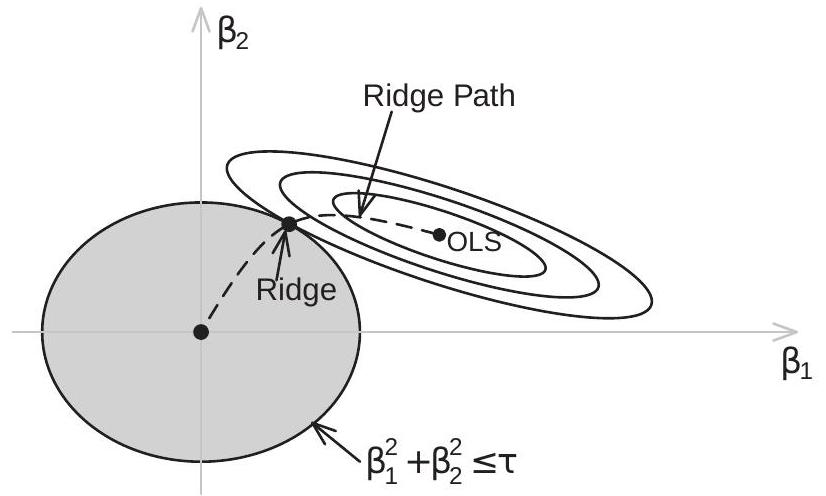
\includegraphics[max width=\textwidth]{2022_11_27_70699ac9776c9435969dg-05}
\end{center}

Figure 29.1: Ridge Regression Dual Minimization Solution

To visualize the constraint problem see Figure $29.1$ which plots an example in $\mathbb{R}^{2}$. The constraint set $\beta^{\prime} \beta \leq \tau$ is displayed as the ball about the origin and the contour sets of the sum of squared errors are displayed as ellipses. The least squares estimator is the center of the ellipses, while the ridge regression estimator is the point on the circle where the contour is tangent. This shrinks the least squares coefficient towards the zero vector. Unlike the Stein estimator, however, it does not shrink along the line segment connecting least squares with the origin, rather it shrinks along a trajectory determined by the degree of correlation between the variables. This trajectory is displayed with the dashed lines, marked as "Ridge path". This is the sequence of ridge regression coefficients obtained as $\lambda$ is varied from 0 to $\infty$. When $\lambda=0$ the ridge estimator equals least squares. For small $\lambda$ the ridge estimator moves slightly towards the origin by sliding along the ridge of the contour set. As $\lambda$ increases the ridge estimator takes a more direct path towards the origin. This is unlike the Stein estimator which shrinks the least squares estimator towards the origin along the connecting line segment. It is straightforward to generalize ridge regression to allow different penalties on different groups of regressors. Take the model

$$
Y=X_{1}^{\prime} \beta_{1}+\cdots+X_{G}^{\prime} \beta_{G}+e
$$

and minimize the SSE subject to the penalty

$$
\lambda_{1} \beta_{1}^{\prime} \beta_{1}+\cdots+\lambda_{G} \beta_{G}^{\prime} \beta_{G} .
$$

The solution is

$$
\widehat{\beta}_{\text {ridge }}=\left(\boldsymbol{X}^{\prime} \boldsymbol{X}+\Lambda\right)^{-1} \boldsymbol{X}^{\prime} \boldsymbol{Y}
$$

where

$$
\Lambda=\operatorname{diag}\left\{\lambda_{1} \boldsymbol{I}_{p_{1}}, \ldots, \lambda_{G} \boldsymbol{I}_{p_{G}}\right\}
$$

This allows some coefficients to be penalized more (or less) than other coefficients. This added flexibility comes at the cost of selecting the ridge parameters $\lambda=\left(\lambda_{1}, \ldots, \lambda_{G}\right)$. One important special case is $\lambda_{1}=0$, thus one group of coefficients are not penalized. With $G=2$ this partitions the coefficients into two groups: penalized and non-penalized.

The most popular method to select the ridge parameter $\lambda$ is cross validation. The leave-one-out ridge regression estimator, prediction errors, and CV criterion are

$$
\begin{aligned}
\widehat{\beta}_{-i}(\lambda) &=\left(\sum_{j \neq i} X_{j} X_{j}^{\prime}+\Lambda\right)^{-1}\left(\sum_{j \neq i} X_{j} Y_{i}\right) \\
\widetilde{e}_{i}(\lambda) &=Y_{i}-X_{i}^{\prime} \widehat{\beta}_{-i}(\lambda) \\
\mathrm{CV}(\lambda) &=\sum_{i=1}^{n} \widetilde{e}_{i}(\lambda)^{2} .
\end{aligned}
$$

The CV-selected ridge parameter $\lambda_{\mathrm{cv}}$ minimizes $\mathrm{CV}(\lambda)$. The cross-validation ridge estimator is calculated using $\lambda_{\mathrm{cv}}$.

In practice it may be tricky to minimize $\mathrm{CV}(\lambda)$. The minimum may occur at $\lambda=0$ (ridge equals least squares), at $\lambda=\infty$ (full shrinkage), or there may be multiple local minima. The scale of the minimizing $\lambda$ depends on the scaling of the regressors and in particular the singular values of $\boldsymbol{X}^{\prime} \boldsymbol{X}$. It can be important to explore CV $(\lambda)$ for very small values of $\lambda$.

As for least squares there is a simple formula to calculate the CV criterion for ridge regression which greatly speeds computation.

Theorem 29.1 The leave-one-out ridge regression prediction errors are

$$
\widetilde{e}_{i}(\lambda)=\left(1-X_{i}^{\prime}\left(\boldsymbol{X}^{\prime} \boldsymbol{X}+\Lambda\right)^{-1} X_{i}\right)^{-1} \widehat{e}_{i}(\lambda)
$$

where $\widehat{e}_{i}(\lambda)=Y_{i}-X_{i}^{\prime} \widehat{\beta}_{\text {ridge }}(\lambda)$ are the ridge regression residuals.

For a proof see Exercise 29.1.

An alternative method for selection of $\lambda$ is to minimize the Mallows criterion which equals

$$
C(\lambda)=\sum_{i=1}^{n} \widehat{e}_{i}(\lambda)^{2}+2 \widehat{\sigma}^{2} \operatorname{tr}\left(\left(\boldsymbol{X}^{\prime} \boldsymbol{X}+\Lambda\right)^{-1}\left(\boldsymbol{X}^{\prime} \boldsymbol{X}\right)\right)
$$

where $\widehat{\sigma}^{2}$ is the variance estimator from least squares estimation. For a derivation of (29.7) see Exercise 29.2. The Mallows-selected ridge parameter $\lambda_{\mathrm{m}}$ minimizes $C(\lambda)$. The Mallows-selected ridge estimator is calculated using $\lambda_{\mathrm{m}}$. $\mathrm{Li}$ (1986) showed that in the normal regression model the ridge estimator with the Mallows-selected ridge parameter is asymptotically equivalent to the infeasible best ridge parameter in terms of regression fit. I am unaware of a similar optimality result for cross-validated-selected ridge estimation.

An important caveat is that the ridge regression estimator is not invariant to rescaling the regressors nor other linear transformations. Therefore it is common to apply ridge regression after applying standardizing transformations to the regressors.

Ridge regression can be implemented in $\mathrm{R}$ with the glmnet command. In Stata, ridge regression is available in the downloadable package lassopack.

\subsection{Statistical Properties of Ridge Regression}
Under the assumptions of the linear regression model it is straightforward to calculate the exact bias and variance of the ridge regression estimator. Take the linear regression model

$$
\begin{aligned}
Y &=X^{\prime} \beta+e \\
\mathbb{E}[e \mid X] &=0 .
\end{aligned}
$$

The bias of the ridge estimator with fixed $\lambda$ is

$$
\operatorname{bias}\left[\widehat{\beta}_{\text {ridge }} \mid \boldsymbol{X}\right]=-\lambda\left(\boldsymbol{X}^{\prime} \boldsymbol{X}+\lambda \boldsymbol{I}_{p}\right)^{-1} \beta \text {. }
$$

Under random sampling its covariance matrix is

$$
\operatorname{var}\left[\widehat{\beta}_{\text {ridge }} \mid \boldsymbol{X}\right]=\left(\boldsymbol{X}^{\prime} \boldsymbol{X}+\lambda \boldsymbol{I}_{p}\right)^{-1}\left(\boldsymbol{X}^{\prime} \boldsymbol{D} \boldsymbol{X}\right)\left(\boldsymbol{X}^{\prime} \boldsymbol{X}+\lambda \boldsymbol{I}_{p}\right)^{-1}
$$

where $\boldsymbol{D}=\operatorname{diag}\left\{\sigma^{2}\left(X_{1}\right), \ldots, \sigma^{2}\left(X_{n}\right)\right\}$ and $\sigma^{2}(X)=\mathbb{E}\left[e^{2} \mid X\right]$. For a derivation of (29.8) and (29.9) see Exercise 29.3. Under cluster or serial dependence the central component modifies in the standard way.

We can measure estimation efficiency by the mean squared error (MSE) matrix

$$
\operatorname{mse}[\widehat{\beta} \mid \boldsymbol{X}]=\mathbb{E}\left[(\widehat{\beta}-\beta)(\widehat{\beta}-\beta)^{\prime} \mid \boldsymbol{X}\right] .
$$

Define $\underline{\sigma}^{2}=\min _{x \in \mathscr{X}} \sigma^{2}(x)$ where $\mathscr{X}$ is the support of $X$.

Theorem 29.2 In the linear regression model, if $0<\lambda<2 \underline{\sigma}^{2} / \beta^{\prime} \beta$,

$$
\operatorname{mse}\left[\widehat{\beta}_{\text {ridge }} \mid \boldsymbol{X}\right]<\operatorname{mse}\left[\widehat{\beta}_{\text {ols }} \mid \boldsymbol{X}\right] .
$$

For a proof see Section $29.23$.

Theorem $29.2$ shows that the ridge estimator dominates the least squares estimator, if $\lambda$ satisfies a specific range of values. This holds regardless of the dimension of $\beta$. Since the upper bound $2 \underline{\sigma}^{2} / \beta^{\prime} \beta$ is unknown, however, it is unclear if feasible ridge regression dominates least squares. The upper bound does not give practical guidance for selection of $\lambda$. Given (29.9) it is straightforward to construct estimators of $V_{\widehat{\beta}}=\operatorname{var}\left[\widehat{\beta}_{\text {ridge }} \mid \boldsymbol{X}\right]$. I suggest the HC3 analog

$$
\widetilde{V}_{\widehat{\beta}}=\left(\boldsymbol{X}^{\prime} \boldsymbol{X}+\lambda \boldsymbol{I}_{p}\right)^{-1}\left(\sum_{i=1}^{n} X_{i} X_{i}^{\prime} \widetilde{e}_{i}(\lambda)^{2}\right)\left(\boldsymbol{X}^{\prime} \boldsymbol{X}+\lambda \boldsymbol{I}_{p}\right)^{-1}
$$

where $\widetilde{e}_{i}(\lambda)$ are the ridge regression prediction errors (29.6). Alternatively, the ridge regression residuals $\widehat{e}_{i}(\lambda)$ can be used but it is unclear how to make an appropriate degree-of-freedom correction. Under clustering or serial dependence the central component of $\widetilde{V}_{\widehat{\beta}}$ can be modified as usual. If the regressors are highly sparse (as in a sparse dummy variable regression) it may be prudent to use the homoskedastic estimator

$$
\widetilde{V}_{\widehat{\beta}}^{0}=\widetilde{\sigma}^{2}(\lambda)\left(\boldsymbol{X}^{\prime} \boldsymbol{X}+\lambda \boldsymbol{I}_{p}\right)^{-1}\left(\boldsymbol{X}^{\prime} \boldsymbol{X}\right)\left(\boldsymbol{X}^{\prime} \boldsymbol{X}+\lambda \boldsymbol{I}_{p}\right)^{-1}
$$

with $\widetilde{\sigma}^{2}(\lambda)=n^{-1} \sum_{i=1}^{n} \widetilde{e}_{i}(\lambda)^{2}$.

Given that the ridge estimator is explicitly biased there are natural concerns about how to interpret standard errors calculated from these covariance matrix estimators. Confidence intervals calculated the usual way will have deficient coverage due to the bias. One answer is to interpret the ridge estimator $\widehat{\beta}_{\text {ridge }}$ and its standard errors similarly to those obtained in nonparametric regression. The estimators and confidence intervals are valid for the pseudo-true projections, e.g. $\beta^{*}=\left(\boldsymbol{X}^{\prime} \boldsymbol{X}+\lambda \boldsymbol{I}_{p}\right)^{-1} \boldsymbol{X}^{\prime} \boldsymbol{X} \beta$, not the coefficients $\beta$ themselves. This is the same interpretation as we use for the projection model and for nonparametric regression. For asymptotically accurate inference on the true coefficients $\beta$ the ridge parameter $\lambda$ could be selected to satisfy $\lambda=o(\sqrt{n})$ analogously to an undersmoothing bandwidth in nonparametric regression.

\subsection{Illustrating Ridge Regression}
\begin{center}
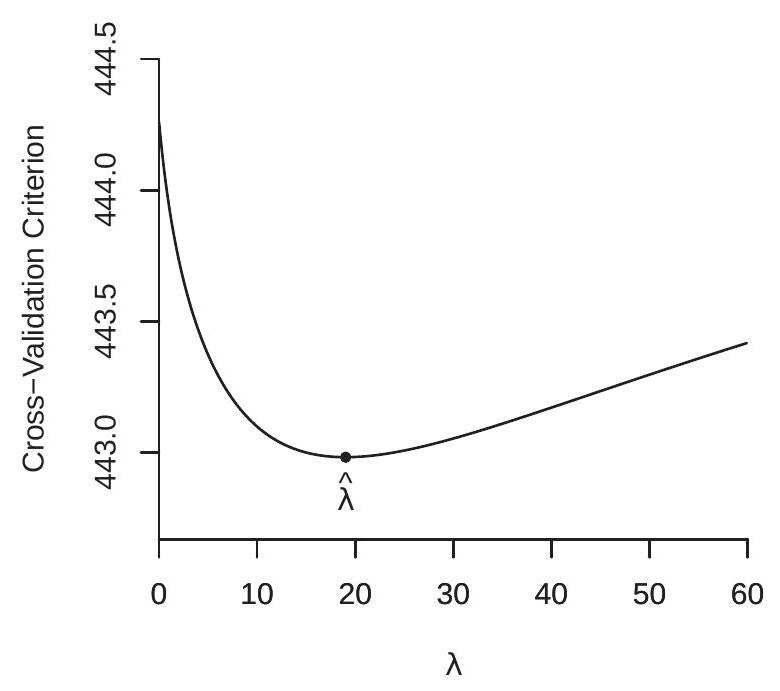
\includegraphics[max width=\textwidth]{2022_11_27_70699ac9776c9435969dg-08}
\end{center}

(a) Cross-Validation Function

\begin{center}
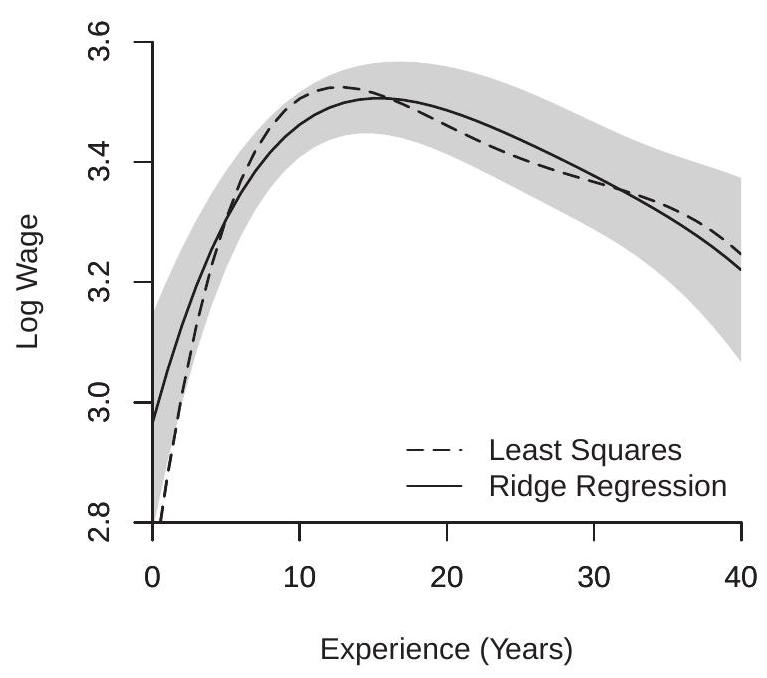
\includegraphics[max width=\textwidth]{2022_11_27_70699ac9776c9435969dg-08(1)}
\end{center}

(b) Estimates of Return to Experience

Figure 29.2: Least Squares and Ridge Regression Estimates of the Return to Experience To illustrate ridge regression we use the CPS dataset with the sample of Asian men with a college education (16 years of education or more) to estimate the experience profile. We consider a fifth-order polynomial in experience for the conditional mean of log wages. We start by standardizing the regressors. We first center experience at its mean, create powers up to order five, and then standardized each to have mean zero and variance one. We estimate the polynomial regression by least squares and by ridge regression, the latter shrinking the five coefficients on experience but not the intercept.

We calculate the ridge parameter by cross-validation. The cross-validation function is displayed in Figure 29.2(a) over the interval [0,60]. Since we have standardized the regressors to have zero mean and unit variance the ridge parameter is scaled comparably with sample size, which in this application is $n=875$. The cross-validation function is uniquely minimized at $\lambda=19$. I use this value of $\lambda$ for the following ridge regression estimation.

Figure 29.2(b) displays the estimated experience profiles. Least squares is displayed by dashes and ridge regression by the solid line. The ridge regression estimate is smoother and more compelling. The grey shaded region are $95 \%$ normal confidence bands centered at the ridge regression estimate, calculated using the HC3 covariance matrix estimator (29.10).

\subsection{Lasso}
In the previous section we learned that ridge regression minimizes the sum of squared errors plus a 2-norm penalty on the coefficient vector. Model selection (e.g. Mallows) minimizes the sum of squared errors plus the 0-norm penalty (the number of non-zero coefficients). An intermediate case uses the 1-norm penalty. This was proposed by Tibshirani (1996) and is known as the Lasso (for Least Absolute Shrinkage and Selection Operator). The least squares criterion with a 1-norm penalty is

$$
\operatorname{SSE}_{1}(\beta, \lambda)=(\boldsymbol{Y}-\boldsymbol{X} \beta)^{\prime}(\boldsymbol{Y}-\boldsymbol{X} \beta)+\lambda \sum_{j=1}^{p}\left|\beta_{j}\right|=\|\boldsymbol{Y}-\boldsymbol{X} \beta\|_{2}^{2}+\lambda\|\beta\|_{1} .
$$

The Lasso estimator is its minimizer

$$
\widehat{\beta}_{\text {Lasso }}=\underset{\beta}{\operatorname{argmin}} \operatorname{SSE}_{1}(\beta, \lambda) .
$$

Except for special cases the solution must be found numerically. Fortunately, computational algorithms are surprisingly simple and fast. An important property is that when $\lambda>0$ the Lasso estimator is welldefined even if $p>n$.

The Lasso minimization problem has the dual constrained minimization problem

$$
\widehat{\beta}_{\text {Lasso }}=\underset{\|\beta\|_{1} \leq \tau}{\operatorname{argmin}} \operatorname{SSE}_{1}(\beta) .
$$

To see that the two problems are the same observe that the constrained minimization problem has the Lagrangian

$$
\min _{\beta}(\boldsymbol{Y}-\boldsymbol{X} \beta)^{\prime}(\boldsymbol{Y}-\boldsymbol{X} \beta)+\lambda\left(\sum_{j=1}^{p}\left|\beta_{j}\right|-\tau\right)
$$

which has first order conditions

$$
-2 \boldsymbol{X}_{j}^{\prime}(\boldsymbol{Y}-\boldsymbol{X} \beta)+\lambda \operatorname{sgn}\left(\beta_{j}\right)=0 .
$$

This is the same as those for minimization of the penalized criterion. Thus the solutions are identical.

\begin{center}
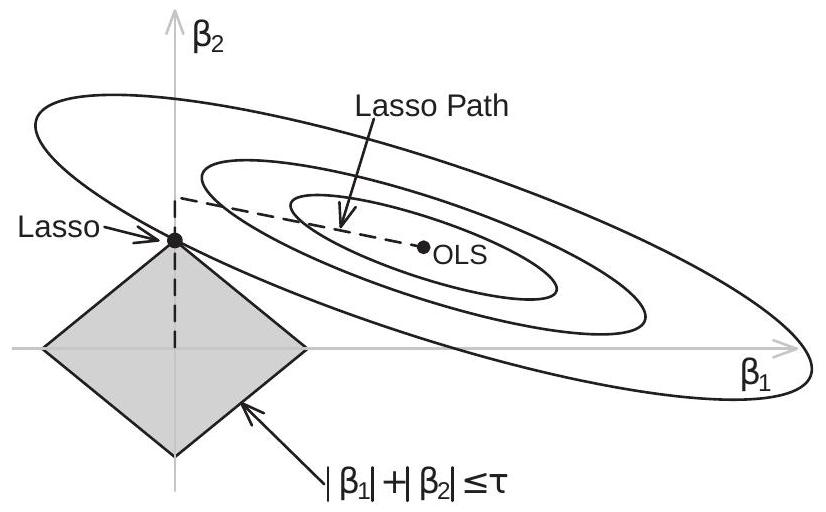
\includegraphics[max width=\textwidth]{2022_11_27_70699ac9776c9435969dg-10}
\end{center}

Figure 29.3: Lasso Dual Minimization Solution

The constraint set $\left\{\|\beta\|_{1} \leq \tau\right\}$ for the dual problem is a cross-polytope resembling a multi-faceted diamond. The minimization problem in $\mathbb{R}^{2}$ is illustrated in Figure 29.3. The sum of squared error contour sets are the ellipses with the least squares solution at the center. The constraint set is the shaded polytope. The Lasso estimator is the intersection point between the constraint set and the largest ellipse drawn. In this example it hits a vertex of the constraint set and so the constrained estimator sets $\widehat{\beta}_{1}=0$. This is a typical outcome in Lasso estimation. Since we are minimizing a quadratic subject to a polytope, solutions tend to be at vertices. This eliminates a subset of the coefficients.

The Lasso path is drawn with the dashed line. This is the sequence of solutions obtained as the constraint set is varied. The solution path has the property that it is a straight line from the least squares estimator to the $y$-axis (in this example), at which point $\beta_{2}$ is set to zero, and then the solution path follows the $y$-axis to the origin. In general, the solution path is linear on segments until a coefficient hits zero, at which point that coefficient is eliminated. In this particular example the solution path shows $\beta_{2}$ increasing while $\beta_{1}$ decreases. Thus while Lasso is a shrinkage estimator it does not shrink individual coefficients monotonically.

It is instructive to compare Figures $29.1$ and $29.3$ which have the same sum of squares contours. The ridge estimator is generically an interior solution with no individual coefficient set to zero, while the Lasso estimator typically sets some coefficients equal to zero. However both estimators follow similar solution paths, following the ridge of the SSE criterion rather than taking a direct path towards the origin.

One case where we can explicitly calculate the Lasso estimates is when the regressors are orthogonal, e.g., $\boldsymbol{X}^{\prime} \boldsymbol{X}=\boldsymbol{I}_{p}$. Then the first order condition for minimization simplifies to

$$
-2\left(\widehat{\beta}_{\text {ols }, j}-\widehat{\beta}_{\text {Lasso }, j}\right)+\lambda \operatorname{sgn}\left(\widehat{\beta}_{\text {Lasso }, j}\right)=0
$$

which has the explicit solution

$$
\widehat{\beta}_{\text {Lasso }, j}=\left\{\begin{array}{cc}
\widehat{\beta}_{\mathrm{ols}, j}-\lambda / 2 & \widehat{\beta}_{\mathrm{ols}, j}>\lambda / 2 \\
0 & \left|\widehat{\beta}_{\mathrm{ols}, j}\right| \leq \lambda / 2 \\
\widehat{\beta}_{\mathrm{ols}, j}+\lambda / 2 & \widehat{\beta}_{\mathrm{ols}, j}<-\lambda / 2
\end{array}\right.
$$

This shows that theLasso estimate is a continuous transformation of the least squares estimate. For small values of the least squares estimate the Lasso estimate is set to zero. For all other values the Lasso estimate moves the least squares estimate towards zero by $\lambda / 2$.

\begin{center}
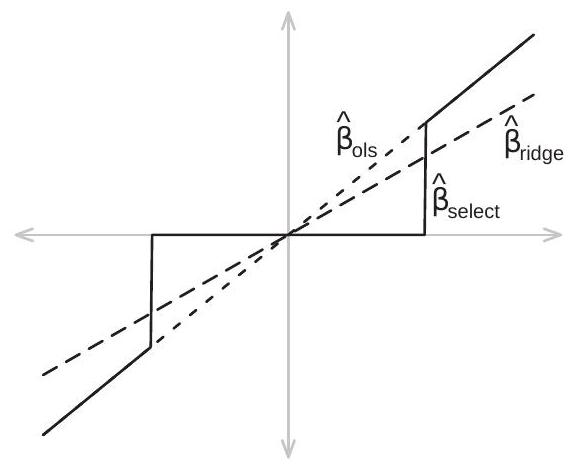
\includegraphics[max width=\textwidth]{2022_11_27_70699ac9776c9435969dg-11}
\end{center}

(a) Selection and Ridge

\begin{center}
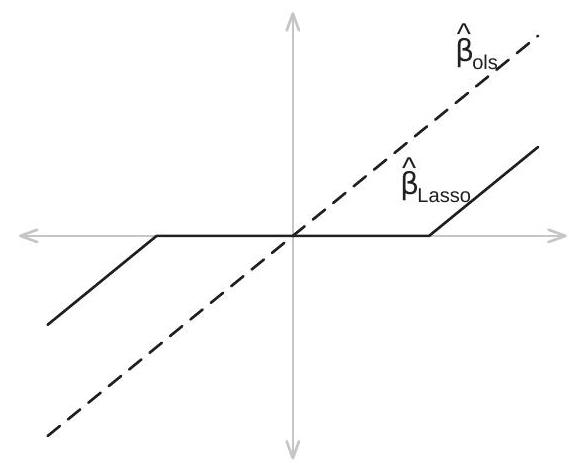
\includegraphics[max width=\textwidth]{2022_11_27_70699ac9776c9435969dg-11(1)}
\end{center}

(b) Lasso

Figure 29.4: Transformations of Least Squares Estimates by Selection, Ridge, and Lasso

It is constructive to contrast this behavior with ridge regression and selection estimation. When $\boldsymbol{X}^{\prime} \boldsymbol{X}=\boldsymbol{I}_{k}$ the ridge estimator equals $\widehat{\beta}_{\text {ridge }}=(1+\lambda)^{-1} \widehat{\beta}_{\text {ols }}$ so shrinks the coefficients towards zero by a common multiple. A selection estimator (for simplicity consider selection based on a homoskedastic $\mathrm{t}$-test with $\widehat{\sigma}^{2}=1$ and critical value $c$ ) equals $\widehat{\beta}_{\text {select }}=\mathbb{1}\left\{\left|\widehat{\beta}_{\text {ols }, j}\right|>c\right\} \widehat{\beta}_{\text {ols }, j}$. Thus the Lasso, ridge, and selection estimates are all transformations of the least squares coefficient estimate. We illustrate these transformations in Figure 29.4. Panel (a) displays the selection and ridge transformations, and panel (b) displays the Lasso transformation.

The Lasso and ridge estimators are continuous functions while the selection estimator is a discontinuous function. The Lasso and selection estimators are thresholding functions, meaning that the function equals zero for a region about the origin. Thresholding estimators are selection estimators because they equal zero when the least squares estimator is sufficiently small. The Lasso function is a "soft thresholding" rule as it is a continuous function with bounded first derivative. The selection estimator is a "hard thresholding" rule as it is discontinuous. Hard thresholding rules tend to have high variance due to the discontinuous transformation. Consequently, we expect the Lasso to have reduced variance relative to selection estimators, permitting overall lower MSE.

As for ridge regression, Lasso is not invariant to the scaling of the regressors. If you rescale a regressor then the penalty has a different meaning. Consequently, it is important to scale the regressors appropriately before applying Lasso. It is conventional to scale all the variables to have mean zero and unit variance.

Lasso is also not invariant to rotations of the regressors. For example, Lasso on $\left(\boldsymbol{X}_{1}, \boldsymbol{X}_{2}\right)$ is not the same as Lasso on $\left(\boldsymbol{X}_{1}-\boldsymbol{X}_{2}, \boldsymbol{X}_{2}\right)$ despite having identical least squares solutions. This is troubling as typically there is no default specification.

Applications of Lasso estimation in economics are growing. Belloni, Chernozhukov and Hansen (2014) illustrate the method using three application: (1) the effect of eminent domain on housing prices in an instrumental variables framework, (2) a re-examination of the effect of abortion on crime using the framework of Donohue and Levitt (2001), (3) a re-examination of the the effect of democracy on growth using the framework of Acemoglu, Johnson, and Robinson (2001). Mullainathan and Spiess (2017) illustrate machine learning using a prediction model for housing prices using characteristics. Oster (2018) uses household scanner data to measure the effect of a diabetes diagnosis on food purchases.

\subsection{Lasso Penalty Selection}
Critically important for Lasso estimation is the penalty $\lambda$. For $\lambda$ close to zero the estimates are close to least squares. As $\lambda$ increases the number of selected variables falls. Picking $\lambda$ induces a trade-off between complexity and parsimony.

It is common in the statistics literature to see coefficients plotted as a function of $\lambda$. This can be used to visualize the trade-off between parsimony and variable inclusion. It does not, however, provide a statistical rule for selection.

The most common selection method is minimization of K-fold cross validation (see Section 28.9). Leave-one-out CV is not typically used as it is computationally expensive. Many programs set the default number of folds as $K=10$, though some authors use $K=5$, while others recommend $K=20$.

K-fold cross validation is an estimator of out-of-sample mean squared forecast error. Therefore penalty selection by minimization of the K-fold criterion is aimed to select models with good forecast accuracy, but not necessarily for other purposes such as accurate inference.

Conventionally, the value of $\lambda$ selected by CV is the value which minimizes the CV criterion. Another popular choice is called the "1se" rule, which is the $\lambda$ which yields the most parsimonious model for $\lambda$ values within one standard error of the minimum. The idea is to select a model similar but more parsimonious than the CV-minimizing choice.

K-fold cross validation is implemented by first randomly dividing the observations into $K$ groups. Consequently the $\mathrm{CV}$ criterion is sensitive to the random sorting. It is therefore prudent to set the random number seed for replicability and to assess sensitivity across initial seeds. In general, selecting a larger value for $K$ reduces this sensitivity.

Asymptotic consistency of CV selection for Lasso estimation has been demonstrated by Chetverikov, Liao, and Chernozhukov (2021).

\subsection{Lasso Computation}
The constraint representation of Lasso is minimization of a quadratic subject to linear inequality constraints. This can be implemented by standard quadratic programming which is computationally simple. For evaluation of the cross-validation function, however, it is useful to compute the entire Lasso path. For this a computationally appropriate method is the modified LARS algorithm. (LARS stands for least angle regression.)

The LARS algorithm produces a path of coefficients starting at the origin and ending at least squares. The sequence corresponds to the sequence of constraints $\tau$ which can be calculated by the absolute sum of the coefficients, but neither these values (nor $\lambda$ ) are used by the algorithm. The steps are as follows.

\begin{enumerate}
  \item Start with all coefficients equal to zero.

  \item Find $X_{j}$ most correlated with $Y$.

  \item Increase $\beta_{j}$ in the direction of correlation.

\end{enumerate}

(a) Compute residuals along the way.

(b) Stop when some other $X_{\ell}$ has the same correlation with the residual as $X_{j}$.

(c) If a non-zero coefficient hits zero, drop from the active set of variables and recompute the joint least squares direction.

\begin{enumerate}
  \setcounter{enumi}{3}
  \item Increase $\left(\beta_{j}, \beta_{\ell}\right)$ in their joint least squares direction until some other $X_{m}$ has the same correlation with the residual.

  \item Repeat until all predictors are in model.

\end{enumerate}

This algorithm produces the Lasso path. The equality between the two is not immediately apparent. The demonstration is tedious so is not shown here.

The most popular computational implementation for Lasso is the R glmnet command in the glmnet package. Penalty selection by K-fold cross validation is implmented by the $\mathrm{cv}$.glmnet command. The latter by default reports the penalty selected by the "1se" rule, and reports the minimizing $\lambda$ as lambda .min. The default number of folds is $K=10$.

In Stata, Lasso is available with the command lasso. By default it selects the penalty by minimizing the K-fold cross validation criterion with $K=10$ folds. Many options are available, including constraining the estimator to penalize only a subset of the coefficients. An alternative downloadable package with many options is lassopack.

\subsection{Asymptotic Theory for the Lasso}
The current distribution theory of Lasso estimation is challenging and mostly focused on convergence rates. The results are derived under sparsity or approximate sparsity conditions, the former restricting the number of non-zero coefficients, and the second restricting how a sparse model can approximate a general parameterization. In this section we provide a basic convergence rate for the Lasso estimator $\widehat{\beta}_{\text {Lasso }}$ under a mild moment bound on the errors and a sparsity assumption on the coefficients.

The model is the high-dimensional projection framework:

$$
\begin{aligned}
Y &=X^{\prime} \beta+e \\
\mathbb{E}[X e] &=0
\end{aligned}
$$

where $X$ is $p \times 1$ with $p>>n$. The true coefficient vector $\beta$ is assumed to be sparse in the sense that only a subset of the elements of $\beta$ are non-zero. For some $\lambda$ let $\widehat{\beta}_{\text {Lasso }}$ be the Lasso estimator which minimizes $\operatorname{SSE}_{1}(\beta, \lambda)$. Define the scaled design matrix $\boldsymbol{Q}_{n}=n^{-1} \boldsymbol{X}^{\prime} \boldsymbol{X}$ and the regression fit

$$
\left(\widehat{\beta}_{\text {Lasso }}-\beta\right)^{\prime} \boldsymbol{Q}_{n}\left(\widehat{\beta}_{\text {Lasso }}-\beta\right)=\frac{1}{n} \sum_{i=1}^{n}\left(X_{i}^{\prime}\left(\widehat{\beta}_{\text {Lasso }}-\beta\right)\right)^{2} .
$$

We provide a bound on the regression fit (29.12), the 1-norm fit $\|\widehat{\beta}-\beta\|_{1}$ and the 2-norm fit $\|\widehat{\beta}-\beta\|_{2}$.

The regression fit (29.12) is similar to measures of fit we have used before, including the integrated squared error (20.22) in series regression and the regression fit $R_{n}(K)$ (equation (28.17)) for evaluation of model selection optimality.

When $p>n$ the matrix $\boldsymbol{Q}_{n}$ is singular. The theory, however, requires that it not be "too singular". What is required is non-singularity of all sub-matrices of $\boldsymbol{Q}_{n}$ corresponding to the non-zero coefficients and not "too many" of the zero coefficients. The specific requirement is rather technical. Partition $\beta=\left(\beta_{0}, \beta_{1}\right)$ where the elements of $\beta_{0}$ are all 0 and the elements of $\beta_{1}$ are non-zero. (This partition is a theoretical device and unknown to the econometrician.) Let $b=\left(b_{0}, b_{1}\right) \in \mathbb{R}^{p}$ be partitioned conformably. Define the cone $B=\left\{b \in \mathbb{R}^{p}:\left\|b_{0}\right\|_{1} \leq 3\left\|b_{1}\right\|_{1}\right\}$. This is the set of vectors $b$ such that the sub-vector $b_{0}$ is not "too large" relative to the sub-vector $b_{1}$.

\section{Assumption 29.1 Restricted Eigenvalue Condition (REC)}
With probability approaching 1 as $n \rightarrow \infty$

$$
\min _{b \in B} \frac{b^{\prime} \boldsymbol{Q}_{n} b}{b^{\prime} b} \geq c^{2}>0 .
$$

To gain some understanding of what the REC means, notice that if the minimum (29.13) is taken without restriction over $\mathbb{R}^{p}$ it equals the smallest eigenvalue of $\boldsymbol{Q}_{n}$. Thus when $p<n$ a sufficient condition for the REC is $\lambda_{\min }\left(\boldsymbol{Q}_{n}\right) \geq c^{2}>0$. Instead, the minimum in (29.13) is calculated only over the cone B. In this sense this calculation is similar to a "restricted eigenvalue" which is the source of its name. The REC takes a variety of forms in the theoretical literautre; Assumption $29.1$ is not the weakest but is the most intuitive. Assumption $29.1$ has been shown to hold under primitive conditions on $X$, including normality and boundedness. See Section 3 of Bickel, Ritov, and Tsybakov (2009) and Section $3.1$ of Belloni, Chen, Chernozhukov, and Hansen (2012).

We provide a rate for the Lasso estimator under the assumption of normal errors. Theorem 29.3 Suppose model (29.11) holds with $p>1$ and Assumption $29.1$ holds. Assume that each regressor has been standardized so that $n^{-1} \boldsymbol{X}_{j}^{\prime} \boldsymbol{X}_{j}=1$ before applying the Lasso. Suppose $e \mid X \sim \mathrm{N}\left(0, \sigma^{2}(X)\right)$ where $\sigma^{2}(x) \leq \bar{\sigma}^{2}<\infty$. For some $C$ sufficiently large set

$$
\lambda=C \sqrt{n \log p}
$$

Then there is $D<\infty$ such that with probability arbitrarily close to 1 ,

$$
\begin{gathered}
\left(\widehat{\beta}_{\text {Lasso }}-\beta\right)^{\prime} \boldsymbol{Q}_{n}\left(\widehat{\beta}_{\text {Lasso }}-\beta\right) \leq D\|\beta\|_{0} \frac{\log p}{n}, \\
\left\|\widehat{\beta}_{\text {Lasso }}-\beta\right\|_{1} \leq D\|\beta\|_{0} \sqrt{\frac{\log p}{n}},
\end{gathered}
$$

and

$$
\left\|\widehat{\beta}_{\text {Lasso }}-\beta\right\|_{2} \leq D\|\beta\|_{0}^{1 / 2} \sqrt{\frac{\log p}{n}} .
$$

For a proof see Section $29.23$.

Theorem $29.3$ presents three convergence rates for the Lasso coefficient estimator $\widehat{\beta}_{\text {Lasso }}$, for the regression fit (29.12), covering the 1-norm, and the 2-norm. These rates depend on the number of non-zero coefficients $\|\beta\|_{0}$, the number of variables $p$, and the sample size $n$. Suppose that $\|\beta\|_{0}$ is fixed. Then the bounds (29.15)-(29.17) are $o(1)$ if $\log p=o(n)$. This shows that Lasso estimation is consistent even for an exponentially large number of variables. The rates, however, allow the number of non-zero coefficients $\|\beta\|_{0}$ to increase with $n$ at the cost of slowing the allowable rate of increase of $p$.

We stated earlier in this section that we had assumed that the coefficient vector $\beta$ is sparse, meaning that only a subset of the elements of $\beta$ are non-zero. This appears in the theory through the 0 -norm $\|\beta\|_{0}$, the number of non-zero coefficients. If all elements of $\beta$ are non-zero then $\|\beta\|_{0}=p$ and the bound (29.15) is $O(p \log p / n)$, which is similar to bound (20.24) for series regression obtained in Theorem 20.7. Instead, the assumption of sparsity enables the Lasso estimator to achieve a much improved rate of convergence.

The key to establishing Theorem $29.3$ is a maximal inequality applied to $\frac{1}{n} \boldsymbol{X}^{\prime} \boldsymbol{e}$. Our proof uses the Gaussian Tail inequality (B.39) which requires the assumption of normality. This follows the analysis of Bickel, Ritov, and Tsybakov (2009), though these authors impose homoskedastic errors, which as shown in Theorem $29.3$ can be replaced by the assumption of bounded heteroskedasticity. Other papers in the statistics literature (see the monograph of Bühlmann and van de Geer (2011)) use instead the assumption of sub-Gaussian tails, which is weaker than normality.

A theory which allows for non-normal heteroskedastic errors has been developed by Belloni, Chen, Chernozhukov, and Hansen (2012). These authors examine an alternative Lasso estimator which adds regresssor-specific weights to the penalty function, with weights equalling the square roots of $n^{-1} \sum X_{j i}^{2} \widehat{e}_{i}^{2}$. They use a maximal inequality based on self-normalization and obtain rates similar to (29.15)-(29.17), though with considerably more complicated regularity conditions. While their specific conditions may not be the weakest possible, their theory shows that the assumption of Gaussian or sub-Gaussian errors is not essential to the convergence rates (29.15)-(29.17). I expect that future research will further clarify the needed conditions. An important limitation of results such as Theorem $29.3$ is the sparsity assumption. It is untestable and counter-intuitive. Researchers in this field frequently use the phrase "imposing sparsity" as if it is something under the control of the theorist - but sparsity is a property of the true coefficients, not a choice of the researcher. Fortunately there are alternatives to the sparsity assumption as we discuss in the following section.

\subsection{Approximate Sparsity}
The theory of the previous section used the strong assumption that the true regression is sparse: only a subset of the coefficients are non-zero, and the convergence rate depends on the cardinality of the nonzero coefficients. However, as shown by Belloni, Chen, Chernozhukov, and Hansen (2012), strict sparsity is not required. Instead, convergence rates similar to those in Theorem $29.3$ hold under the assumption of approximate sparsity.

Once again take the high-dimensional regression model (29.11) but do not assume that $\beta$ necessarily has a sparse structure. Instead, view a sparse model as an approximation. For each integer $K>0$ let $B_{K}=$ $\left\{b \in \mathbb{R}^{p}:\|b\|_{0}=K\right\}$ be the set of vectors with $K$ non-zero elements. Define the best sparse approximation

$$
\beta_{K}=\underset{b \in B_{K}}{\operatorname{argmin}}\left\|\boldsymbol{Q}_{n}(\beta-b)\right\|_{\infty}
$$

with associated approximation error

$$
r_{K}=\left\|\boldsymbol{Q}_{n}\left(\beta-\beta_{K}\right)\right\|_{\infty} .
$$

Assumption 29.2 Approximate Sparsity. For some $s>1, r_{K}=O\left(K^{-s}\right)$.

Assumption $29.2$ states that the approximation error of the sparse approximation decreases at a power law rate. In Section $20.8$ and Theorem $20.1$ we learned that approximations similar to Assumption $29.2$ hold for polynomial and spline series regressions with bounded regressors if the true regression function has a uniform $s^{t h}$ derivative. The primary difference is that series regression requires that the econometrician knows how to order the regressors while Assumption $29.2$ does not impose a specific ordering. In this sense Assumption $29.2$ is weaker than the approximation conditions of Section 20.8.

Belloni, Chen, Chernozhukov, and Hansen (2012) show that convergence results similar to Theorem 29.3 hold under the approximate sparsity condition of Assumption 29.2. The convergence rates are slowed and depend on the approximation exponent $s$. As $s \rightarrow \infty$ the convergence rates approach those under the assumption of sparsity. The reason is that as $s$ increases the regression function can be approximated with a smaller number $K$ of non-zero coefficients. Their results show that exact sparsity is not required for Lasso estimation, rather what is needed is approximation properties similar to those used in series regression theory.

The approximate sparsity condition fails when the regressors cannot be easily ordered. Suppose, for example, that $\boldsymbol{Q}_{n}=\boldsymbol{I}_{p}$ and all elements of $\beta$ have common value $\delta$. In this case $r_{K}=\delta$ which does not decrease with $K$. In this context Assumption $29.2$ does not hold and the convergence results of Belloni, Chen, Chernozhukov, and Hansen (2012) do not apply.

\subsection{Elastic Net}
The difference between Lasso and ridge regression is that the Lasso uses the 1-norm penalty while ridge uses the 2-norm penalty. Since both procedures have advantages it seems reasonable that further improvements may be obtained by a compromise. Taking a weighted average of the penalties we obtain the Elastic Net criterion

$$
\operatorname{SSE}(\beta, \lambda, \alpha)=(\boldsymbol{Y}-\boldsymbol{X} \beta)^{\prime}(\boldsymbol{Y}-\boldsymbol{X} \beta)+\lambda\left(\alpha\|\beta\|_{2}^{2}+(1-\alpha)\|\beta\|_{1}\right)
$$

with weight $0 \leq \alpha \leq 1$. This includes Lasso $(\alpha=0)$ and ridge regression $(\alpha=1)$ as special cases. For small but positive $\alpha$ the constraint sets are similar to "rounded" versions of the Lasso constraint sets.

Typically the parameters $(\alpha, \lambda)$ are selected by joint minimization of the K-fold cross-validation criterion. Since the elastic net penalty is linear-quadratic the solution is computationally similar to Lasso.

Elastic net can be implemented in R with the glmnet command. In Stata use elasticnet or the downloadable package lassopack.

\subsection{Post-Lasso}
The Lasso estimator $\widehat{\beta}_{\text {Lasso }}$ simultaneously selects variables and shrinks coefficients. Shrinkage introduces bias into estimation. This bias can be reduced by applying least squares after Lasso selection. This is known as the Post-Lasso estimator.

The procedure takes two steps. First, estimate the model $Y=X^{\prime} \beta+e$ by Lasso. Let $X_{S}$ denote the variables in $X$ which have non-zero coefficients in $\widehat{\beta}_{\text {Lasso }}$. Let $\beta_{S}$ denote the corresponding coefficients in $\beta$. Second, the coefficient $\beta_{S}$ is estimated by least squares, thus $\widehat{\beta}_{S}=\left(\boldsymbol{X}_{S}^{\prime} \boldsymbol{X}_{S}\right)^{-1}\left(\boldsymbol{X}_{S}^{\prime} \boldsymbol{Y}\right)$. This is the Post-Lasso least squares estimator. Belloni and Chernozhukov (2013) provide conditions under which the post-Lasso estimator has the same convergence rates as the Lasso estimator.

The post-Lasso is a hard thresholding or post-model-selection estimator. Indeed, when the regressors are orthogonal the post-Lasso estimator precisely equals a selection estimator, transforming the least squares coefficient estimates using the hard threshold function displayed in Figure 29.4(a). Consequently, the post-Lasso estimator inherits the statistical properties of PMS estimators (see Sections $28.16$ and 28.17), including high variance and non-standard distributions.

\subsection{Regression Trees}
Regression trees were introduced by Breiman, Friedman, Olshen, and Stone (1984), and are also known by the acronym CART for Classification and Regression Trees. A regression tree is a nonparametric regression using a large number of step functions. The idea is that with a sufficiently large number of split points, a step function can approximate any function. Regression trees may be especially useful when there are a combination of continuous and discrete regressors so that traditional kernel and series methods are challenging to implement.

Regression trees can be thought of as a $0^{t h}$-order spline with free knots. They are also similar to threshold regression with intercepts only (no slope coefficients) and a very large number of thresholds.

The goal is to estimate $m(x)=\mathbb{E}[Y \mid X=x]$ for scalar $Y$ and vector $X$. The elements of $X$ can be continuous, binary, or ordinal. If a regressor is categorical is should be first transformed to a set of binary variables.

The literature on regression trees has developed some colorful language to describe the tools based on the metaphor of a living tree. 1. A subsample is a branch.

\begin{enumerate}
  \setcounter{enumi}{1}
  \item Terminal branches are nodes or leaves.

  \item Increasing the number of branches is growing a tree.

  \item Decreasing the number of branches is pruning a tree.

\end{enumerate}

The basic algorithm starts with a single branch. Grow a large tree by sequentially splitting the branches. Then prune back using an information criterion. The goal of the growth stage is to develop a rich datadetermined tree which has small estimation bias. Pruning back is an application of backward stepwise regression with the goal of reducing over-parameterization and estimation variance.

The regression tree algorithm makes extensive use of the regression sample split algorithm. This is a simplified version of threshold regression (Section 23.7). The method uses NLLS to estimate the model

$$
\begin{aligned}
Y &=\mu_{1} \mathbb{1}\left\{X_{d} \leq \gamma\right\}+\mu_{2} \mathbb{1}\left\{X_{d}>\gamma\right\}+e \\
\mathbb{E}[e \mid X] &=0
\end{aligned}
$$

with the index $d$ and parameter $\gamma$ as free parameters ${ }^{2}$. The NLLS criterion is minimized over $(d, \gamma)$ by grid search. The estimates produce a sample split. The regression tree algorithm applies sequential sample splitting to make a large number of splits, each on a sub-sample of observations.

The basic growth algorithm is as follows. The observations are $\left\{Y_{i}, X_{1 i}, \ldots, X_{k i}: i=1, \ldots, n\right\}$.

\begin{enumerate}
  \item Select a minimum node size $N_{\min }$ (say 5). This is the minimal number of observations on each leaf.

  \item Sequentially apply regression sample splits.

\end{enumerate}

(a) Apply the regression sample split algorithm to split each branch into two sub-branches, each with size at least $N_{\min }$.

(b) On each sub-branch $b$ :

i. Take the sample mean $\widehat{\mu}_{b}$ of $Y_{i}$ for observations on the sub-branch.

ii. This is the estimator of the regression function on this sub-branch.

iii. The residuals on the sub-branch are $\widehat{e}_{i}=Y_{i}-\widehat{\mu}_{b}$.

(c) Select the branch whose split most reduces the sum of squared errors.

(d) Split this branch into two branches. Make no other split.

(e) Repeat (a)-(d) until each branch cannot be further split. The terminal (unsplit) branches are the leaves.

After the growth algorithm has been run, the estimated regression is a multi-dimensional step function with a large number of branches and leaves.

The basic pruning algorithm is as follows.

\begin{enumerate}
  \item Define the Mallows-type information criterion
\end{enumerate}

$$
C=\sum_{i=1}^{n} \widehat{e}_{i}^{2}+\alpha N
$$

where $N$ is the number of leaves and $\alpha$ is a penalty parameter.

${ }^{2}$ If $X_{d} \in\{0,1\}$ is binary then $\gamma=0$ is fixed. 2. Compute the criterion $C$ for the current tree.

\begin{enumerate}
  \setcounter{enumi}{2}
  \item Use backward stepwise regression to reduce the number of leaves:
\end{enumerate}

(a) Identify the leaf whose removal most decreases $C$.

(b) Prune (remove) this leaf.

(c) If there is no leaf whose removal decreases $C$ then stop pruning.

(d) Otherwise, repeat (a)-(c).

The penalty parameter $\alpha$ is typically selected by K-fold cross-validation. The Mallows-type criterion is used because of its simplicity, but to my knowledge does not have a theoretical foundation for regression tree penalty selection.

The advantage of regression trees is that they provide a highly flexible nonparametric approximation. Their main use is prediction. One disadvantage of regression trees is that the results are difficult to interpret as there are no regression coefficients. Another disadvantage is that the fitted regression $\widehat{m}(x)$ is a discrete step function, which may be a crude approximation when $m(x)$ is continuous and smooth. To obtain a good approximation a regression tree may require a high number of leaves which can result in a non-parsimonious model with high estimation variance.

The sampling distribution of regression trees is difficult to derive, in part because of the strong correlation between the placement of the sample splits and the estimated means. This is similar to the problems associated with post-model-selection. (See Sections $28.16$ and 28.17.) A method which breaks this dependence is the honest tree proposal of Wager and Ather (2018). Split the sample into two halves $A$ and $B$. Use the $A$ sample to place the splits and the $B$ sample to do within-leaf estimation. While reducing estimation efficiency (the sample is effectively halved) the estimated conditional mean will not be distorted by the correlation between the estimated splits and means.

Regression trees algorithms are implemented in the R package rpart.

\subsection{Bagging}
Bagging (bootstrap aggregating) was introduced by Breiman (1996) as a method to reduce the variance of a predictor. We focus here on its use for estimation of a conditional expectation. The basic idea is simple. You generate a large number $B$ of bootstrap samples, estimate your regression model on each bootstrap sample, and take the average of the bootstrap regression estimates. The average of the bootstrap estimates is the bagging estimator of the CEF.

Bagging is believed to be useful when the CEF estimator has low bias but high variance. This occurs for hard thresholding estimators such as regression trees, model selection, and post-Lasso. Bagging is a smoothing operation which reduces variance. The resulting bagging estimator can have lower MSE as a result. Bagging is believed to be less useful for estimators with high bias, as bagging may exaggerate the bias.

We first describe the estimation algorithm. Let $m(x)=\mathbb{E}[Y \mid X=x]$ be the CEF and $\widehat{m}(x)$ an estimator such as a regression tree. Let $\widehat{m}_{b}^{*}(x)$ be the same estimator constructed on a bootstrap sample. The bagging estimator of $m(x)$ is

$$
\widehat{m}_{\text {bag }}(x)=\frac{1}{B} \sum_{B=1}^{b} \widehat{m}_{b}^{*}(x)
$$

As $B$ increases this converges in bootstrap probability to the ideal bagging estimator $\mathbb{E}^{*}\left[\widehat{m}^{*}(x)\right]$.

To understand the bagging process we use an example from Bühlmann and Yu (2002). As in Section $28.16$ suppose that $\widehat{\theta} \sim \mathrm{N}(\theta, 1)$ and consider a selection estimator based on a $5 \%$ test, $\widehat{\theta}_{\mathrm{pms}}=\widehat{\theta} \mathbb{1}\left\{\widehat{\theta}^{2} \geq c\right\}=$ $h(\widehat{\theta})$ where $c=3.84$ and $h(t)=t \mathbb{1}\left\{t^{2} \geq c\right\}$. Applying Theorem 28.17, equation (28.38), we can calculate that $\mathbb{E}\left[\widehat{\theta}_{\mathrm{pms}}\right]=g(\theta)$ where $g(t)=t\left(1-F_{3}\left(c, t^{2}\right)\right)$ and $F_{r}(x, \lambda)$ is the non-central chi-square distribution function ${ }^{3}$. This representation is not intuitive so it is better to visualize its graph. The functions $h(t)$ and $g(t)$ are plotted in Figure 29.5(a). The selection function $h(t)$ is identical to the plot in Figure 29.4(a). The function $g(t)$ is a smoothed version of $h(t)$, everywhere continuous and differentiable.

Suppose that the bagging estimator is constructed using the parametric bootstrap $\widehat{\theta}^{*} \sim \mathrm{N}(\widehat{\theta}, 1)$. The bootstrap selection estimator is $\widehat{\theta}_{\mathrm{pms}}^{*}=h\left(\widehat{\theta}^{*}\right)$. It follows that the bagging estimator is $\widehat{\theta}_{\mathrm{bag}}=\mathbb{E}^{*}\left[\widehat{\theta}_{\mathrm{pms}}^{*}\right]=$ $\mathbb{E}^{*}\left[h\left(\widehat{\theta}^{*}\right)\right]=g(\widehat{\theta})$. Thus while the selection estimator $\widehat{\theta}_{\mathrm{pms}}=h(\widehat{\theta})$ is the hard threshold transformation $h(t)$ applied to $\widehat{\theta}$, the bagging estimator $\widehat{\theta}_{\mathrm{bag}}=g(\widehat{\theta})$ is the smoothed transformation $g(t)$ applied to $\widehat{\theta}$. Thus Figure 29.5(a) displays how $\widehat{\theta}_{\mathrm{pms}}$ and $\hat{\theta}_{\mathrm{bag}}$ are transformations of $\widehat{\theta}$, with the bagging estimator a smooth transformation rather than a hard threshold transformation.

\begin{center}
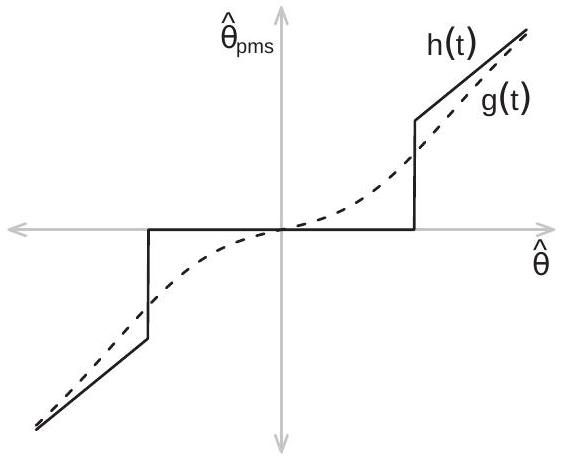
\includegraphics[max width=\textwidth]{2022_11_27_70699ac9776c9435969dg-20}
\end{center}

(a) Selection and Bagging Transformations

\begin{center}
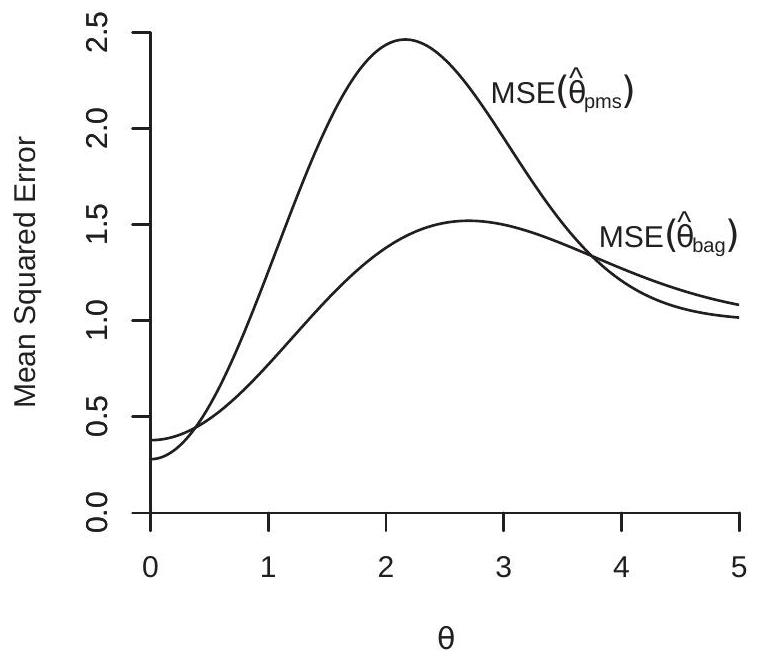
\includegraphics[max width=\textwidth]{2022_11_27_70699ac9776c9435969dg-20(1)}
\end{center}

(b) MSE of Selection and Bagging Estimators

Figure 29.5: Bagging and Selection

Bühlmann and Yu (2002) argue that smooth transformations generally have lower variances than hard threshold transformations, and thus argue that $\widehat{\theta}_{\text {bag }}$ will generally have lower variance than $\widehat{\theta}_{\mathrm{pms}}$. This is difficult to demonstrate as a general principle but seems satisfied in specific examples. For our example we display ${ }^{4}$ in Figure 29.5(b) the MSE of the selection estimator $\widehat{\theta}_{\mathrm{pms}}$ and its bagged verion $\widehat{\theta}_{\text {bag }}$ as functions of $\theta$. As we learned in Section 28.16, the MSE of the selection estimator $\widehat{\theta}_{\text {pms }}$ is a humpshaped function of $\theta$. In Figure 29.5(b) we can see that the MSE of the bagged estimator is considerably reduced relative to the selection estimator for most values of $\theta$. The reduction in MSE is greatest in the region where the MSE of $\widehat{\theta}_{\text {pms }}$ is greatest. Bühlmann and Yu (2002) also calculate that most of this MSE reduction is due to a reduction in the variance of the bagged estimator.

The most common application of bagging is to regression trees. Trees have a similar structure to our example selection estimator $\widehat{\theta}_{\mathrm{pms}}$ and are therefore expected to have a similar reduction in estimation variance and MSE relative to regression tree estimation.

${ }^{3}$ Bühlmann and Yu (2002), Proposition 2.2, provide an alternative representation using the normal cdf and pdf functions.

${ }^{4}$ For $\widehat{\theta}_{\text {pms }}$ the MSE is calculated using Theorem 28.10. For $\widehat{\theta}_{\text {bag }}$ the MSE is calculated by numerical integration. One convenient by-product of bagging is a CV proxy called the out-of-bag (OOB) prediction error. A typical nonparametric bootstrap sample contains about $63 \%$ of the original observations, meaning that about $37 \%$ of the observations are not present in that bootstrap sample. Therefore a bootstrap estimate of the regression function $m(x)$ constructed on this bootstrap sample has "left out" about $37 \%$ of the observations, meaning that valid prediction errors can be calculated on these "left out" observations. Alternatively, for any given observation $i$, out of the $B$ bootstrap samples about $0.63 \times B$ samples will contain this observation and about $0.37 \times B$ samples will not include this observation. The bagging "leave $i$ out" estimator $\widehat{m}_{-i}(x)$ of $m(x)$ is obtained by averaging just this second set (the $37 \%$ which exclude the observation). The out-of-bag error is $\widetilde{e}_{i}=Y_{i}-\widehat{m}_{-i}\left(X_{i}\right)$. The out-of-bag CV criterion is $\sum_{i=1}^{n} \widetilde{e}_{i}^{2}$. This can be used as an estimator of out-of-sample MSFE and can be used to compare and select models.

Wager, Hastie, and Efron (2014) propose estimators of $V_{n}(x)=\operatorname{var}\left[\widehat{m}_{\text {bag }}(x)\right]$. Let $N_{i b}$ denote the number of times observation $i$ appears in the bootstrap sample $b$ and $N_{i}=B^{-1} \sum_{b=1}^{B} N_{i b}$. The infinitesimal jackknife estimator of $V_{n}$ is

$$
\widehat{V}_{n}(x)=\sum_{i=1}^{n} \operatorname{cov}^{*}\left(N_{i}, \widehat{m}_{\text {bag }}(x)\right)^{2}=\sum_{i=1}^{n}\left(\frac{1}{B} \sum_{b=1}^{B}\left(N_{i b}-N_{i}\right)\left(\widehat{m}_{b}^{*}(x)-\widehat{m}_{\text {bag }}(x)\right)\right)^{2} .
$$

This variance estimator is based on Efron (2014).

While Breiman's proposal and most applications of bagging are implemented using the nonparametric bootstrap, an alternative is to use subsampling. A subsampling estimator is based on sampling without replacement rather than with replacement as done in the conventional bootstrap. Samples of size $s<n$ are drawn from the original sample and used to construct the estimator $\widehat{m}_{b}^{*}(x)$. Otherwise the methods are identical. It turns out that it is somewhat easier to develop a distribution theory for bagging under subsampling, so a subsampling assumption is frequently employed in theoretical treatments.

\subsection{Random Forests}
Random forests, introduced by Breiman (2001), are a modification of bagged regression trees. The modification is designed to reduce estimation variance. Random forests are popular in machine learning applications and have effectively displaced simple regression trees.

Consider the procedure of applying bagging to regression trees. Since bootstrap samples are similar to one another the estimated bootstrap regression trees will also be similar to one another, particularly in the sense that they tend to have the splits based on the same variables. This means that conditional on the sample the bootstrap regression trees are positively correlated. This correlation means that the variance of the bootstrap average remains high even when the number of bootstrap replications $B$ is large. The modification proposed by random forests is to decorrelate the bootstrap regression trees by introducing extra randomness. This decorrelation reduces the variance of the bootstrap average, thereby reducing its MSE.

The basic random forest algorithm is as follows. The recommended defaults are taken from the description in Hastie, Tibshirani, and Friedman (2008).

\begin{enumerate}
  \item Pick a minimum leaf size $N_{\min }$ (default $=5$ ), a minimal split fraction $\alpha \in[0,1$ ), and a sampling number $m<p$ (default $=p / 3$ ).

  \item For $b=1, \ldots, B$ :

\end{enumerate}

(a) Draw a nonparametric bootstrap sample.

(b) Grow a regression tree on the bootstrap sample using the following steps: i. Select $m$ variables at random from the $p$ regressors.

ii. Among these $m$ variables, pick the one which produces the best regression split, where each split subsample has at least $N_{\min }$ observations and at least a fraction $\alpha$ of the observations in the branch.

iii. Split the bootstrap sample accordingly.

(c) Stop when each leaf has between $N_{\min }$ and $2 N_{\min }-1$ observations.

(d) Set $\widehat{m}_{b}(x)$ as the sample mean of $Y$ on each leaf of the bootstrap tree.

\begin{enumerate}
  \setcounter{enumi}{2}
  \item $\widehat{m}_{\mathrm{rf}}(x)=B^{-1} \sum_{B=1}^{b} \widehat{m}_{b}(x)$.
\end{enumerate}

Using randomization to reduce the number of variables from $p$ to $m$ at each step alters the tree structure and thereby reduces the correlation between the bootstrapped regression trees. This reduces the variance of the bootstrap average.

The infinitesimal jackknife (29.18) can be used for variance and standard error estimation, as discussed in Wager, Hastie, and Efron (2014).

While random forests are popular in applications, a distributional theory has been slow to develop. Some of the more recent results have made progress by focusing on random forests generated by subsampling rather than bootstrap (see the discussion at the end of the previous section).

A variant proposed by Wager and Athey (2018) is to use honest trees (see the discussion at the end of Section 29.15) to remove the dependence between the sample splits and the sample means.

Consistency and asymptotic normality has been established by Wager and Athey (2018). They assume that the conditional expectation and variance are Lipschitz-continuous in $x, X \sim U[0,1]^{p}$, and $p$ is fixed ${ }^{5}$. They assume that the random forest is created by subsampling, estimated by honest trees, and that the minimal split fraction satisfies $0<\alpha \leq 0.2$. Under these conditions they establish that pointwise in $x$

$$
\frac{\widehat{m}_{\mathrm{rf}}(x)-m(x)}{\sqrt{V_{n}(x)}} \underset{d}{\longrightarrow} \mathrm{N}(0,1)
$$

for some variance sequence $V_{n}(x) \rightarrow 0$. These results justify inference for random forest estimation of the regression function and standard error calculation. The asymptotic distribution does not contain a bias component, indicating that the estimator is undersmoothed. The Wager-Athey conditions for asymptotic normality are surprisingly weak. The theory does not give insight, however, into the convergence rate of the estimator. The essential idea of the result is as follows. The splitting algorithm and restrictions ensure that the regressor space is (in a rough sense) evenly split into $N \sim n^{\gamma}$ leaves which grows at a power rate. This ensures that the estimator is asymptotically unbiased. With suitable control over $\gamma$ the squared bias can be made smaller than the variance. The assumption that $\alpha>0$ ensures that the number of observations per leaf increases with $n$. When combined with the honest tree construction, this ensures asymptotic normality of the estimator.

Furthermore, Wager and Athey (2018) assert (but do not provide a proof) that the variance $V_{n}(x)$ can be consistently estimated by the infinitesimal jackknife (29.18), in the sense that $\widehat{V}_{n}(x) / V_{n}(x) \underset{p}{\longrightarrow} 1$.

The standard computational implementation of random forests is the R randomForest command.

\section{$29.18$ Ensembling}
Ensembling is the term used in machine learning for model averaging across machine learning algorithms. Ensembling is popular in applied machine learning.

${ }^{5}$ The authors claim that the uniform distribution assumption on $X$ can be replaced by the condition that the joint density is bounded away from 0 and infinity. Suppose you have a set of estimators (e.g., CV selection, James-Stein shrinkage, JMA, SBIC, PCA, kernel regression, series regression, ridge regression, Lasso, regression tree, bagged regression tree, and random forest). Which should you use? It is reasonable to expect that one method may work well with some types of data and other methods may work well with other types of data. The principle of model averaging suggests that you can do better by taking a weighted average rather than just selecting one.

We discussed model averaging models in Sections 28.26-28.31. Ensembling for machine learning can use many of the same methods. One popular method known as stacking is the same as Jackknife Model Averaging discussed in Section 28.29. This selects the model averaging weights by minimizing a cross-validation criterion, subject to the constraint that the weights are non-negative and sum to one.

Unfortunately, the theoretical literature concerning ensembling is thin. Much of the advice concerning specific methods is based on empirical performance.

\section{$29.19$ Lasso IV}
Belloni, Chen, Chernozhukov, and Hansen (2012) propose Lasso for estimation of the reduced form of an instrumental variables regression.

The model is linear IV

$$
\begin{aligned}
Y &=X^{\prime} \beta+e \\
\mathbb{E}[e \mid Z] &=0 \\
X &=\Gamma^{\prime} Z+U \\
\mathbb{E}[U \mid Z] &=0
\end{aligned}
$$

where $\beta$ is $k \times 1$ (fixed) and $\Gamma$ is $p \times n$ with $p$ large. If $p>n$ the 2SLS estimator equals least squares. If $p<n$ but large the 2SLS estimator suffers from the "many instruments" problem. The authors' recommendation is to estimate $\Gamma$ by Lasso or post-Lasso 6 .

The reduced form equations for the endogenous regressors are $X_{j}=\gamma_{j}^{\prime} Z+U_{j}$. Each is estimated separately by Lasso yielding coefficient estimates $\widehat{\gamma}_{j}$ which are stacked into the matrix $\widehat{\Gamma}_{\text {Lasso }}$ and used to form the predicted values $\widehat{\boldsymbol{X}}_{\text {Lasso }}=Z \widehat{\Gamma}_{\text {Lasso }}$. The Lasso IV estimator is

$$
\widehat{\beta}_{\text {Lasso-IV }}=\left(\widehat{\boldsymbol{X}}_{\text {Lasso }}^{\prime} \boldsymbol{X}\right)^{-1}\left(\widehat{\boldsymbol{X}}_{\text {Lasso }}^{\prime} \boldsymbol{Y}\right) .
$$

The paper discusses alternative formulations. One is obtained by split-sample estimation as in Angrist and Krueger (1995) (see Section 12.14). Divide the sample randomly into two independent halves $A$ and $B$. Use $A$ to estimate the reduce form equations by Lasso. Then use $B$ to estimate the structural coefficient $\beta$. Specifically, using sample $A$ construct the Lasso coefficient estimate matrix $\widehat{\Gamma}_{\text {Lasso, } A}$. Combine this with sample $B$ to create the predicted values $\widehat{\boldsymbol{X}}_{\text {Lasso }, B}=Z_{B} \widehat{\Gamma}_{\text {Lasso, } A}$. Finally, using $B$ construct the estimator

$$
\widehat{\beta}_{\text {Lasso }, B}=\left(\widehat{\boldsymbol{X}}_{\text {Lasso }, B}^{\prime} \boldsymbol{X}_{B}\right)^{-1}\left(\widehat{\boldsymbol{X}}_{\text {Lasso }, B}^{\prime} \boldsymbol{Y}_{B}\right) .
$$

We can reverse the procedure. Use $B$ to estimate the reduced form coefficient matrix $\widehat{\Gamma}_{\text {Lasso }, B}$ by Lasso and use $A$ to estimate the structural coefficient, thus $\widehat{\boldsymbol{X}}_{\text {Lasso, } A}=\boldsymbol{Z}_{A} \widehat{\Gamma}_{\text {Lasso, } B}$. The moments are averaged to obtain the Lasso SSIV estimator

$$
\widehat{\beta}_{\text {Lasso-SSIV }}=\left(\widehat{\boldsymbol{X}}_{\text {Lasso }, B}^{\prime} \boldsymbol{X}_{B}+\widehat{\boldsymbol{X}}_{\text {Lasso }, A}^{\prime} \boldsymbol{X}_{A}\right)^{-1}\left(\widehat{\boldsymbol{X}}_{\text {Lasso }, B}^{\prime} \boldsymbol{Y}_{B}+\widehat{\boldsymbol{X}}_{\text {Lasso }, A}^{\prime} \boldsymbol{Y}_{A}\right) .
$$

${ }^{6}$ As they discuss, any machine learning estimator can be used, though the specific assumptions listed in their paper are for Lasso estimation. In later work (see Section 29.22) the authors describe $\widehat{\beta}_{\text {Lasso, } B}$ as a "sample split" and $\widehat{\beta}_{\text {Lasso-SSIV }}$ as a "cross-fit" estimator.

Using the asymptotic theory for Lasso estimation the authors show that these estimators are equivalent to estimation using the infeasible instrument $W=\Gamma^{\prime} Z$.

Theorem 29.4 Under the Assumptions listed in Theorem 3 of Belloni, Chen, Chernozhukov, and Hansen (2012), including

$$
\|\Gamma\|_{0} \frac{\log p}{\sqrt{n}} \rightarrow 0,
$$

then

$$
\left(\boldsymbol{Q}^{-1} \Omega \boldsymbol{Q}^{-1}\right) \sqrt{n}\left(\widehat{\beta}_{\text {Lasso-IV }}-\beta\right) \underset{d}{\rightarrow} \mathrm{N}\left(0, \boldsymbol{I}_{k}\right)
$$

where $\boldsymbol{Q}=\mathbb{E}\left[W W^{\prime}\right], \Omega=\mathbb{E}\left[W W^{\prime} e^{2}\right]$, and $W=\Gamma^{\prime} Z$. Furthermore, the standard covariance matrix estimators are consistent for the asymptotic covariance matrix. The same distribution result holds for $\widehat{\beta}_{\text {Lasso-SSIV }}$ under the assumptions listed in their Theorem 7. In particular, (29.19) is replaced by

$$
\|\Gamma\|_{0} \frac{\log p}{n} \rightarrow 0 .
$$

For a sketch of the proof see Section $29.23$.

Equation (29.19) requires that the reduced form coefficient $\Gamma$ is sparse in the sense that the number of non-zero reduced form coefficients $\|\Gamma\|_{0}$ grows more slowly than $\sqrt{n}$. This allows for $p$ to grow exponentially with $n$ but at a somewhat slower rate than allowed by Theorem 29.3. Condition (29.19) is one of the key assumptions needed for the distribution result (29.20).

For Lasso SSIV, equation (29.21) replaces (29.19). This rate condition is weaker, allowing $p$ to grow at the same rate as for regression estimation. The difference is due to the split-sample estimation, which breaks the dependence between the reduced form coefficient estimates and the second-stage structural estimates. There are two interpretable implications of the difference between (29.19) and (29.21). First, a direct implication is that Lasso SSIV allows for larger number of variables $p$. Second, an indirect implication is that for any set of variables, Lasso SSIV will have reduced bias relative to Lasso IV. Both interpretations suggest that Lasso SSIV is the preferred estimator.

Belloni, Chen, Chernozhukov, and Hansen (2012) extend Theorem $29.4$ to allow for approximate sparsity as in Section $29.12$ at the cost of more restrictive rate conditions.

An important disadvantage of the split-sample and cross-fit estimators is that they depend on the random sorting of the observations into the samples $A$ and $B$. Consequently, two researchers will obtain two different estimators. Furthermore, the split-sample estimators use $n / 2$ observations rather than $n$, which may impact finite-sample performance. A deduction is that the split-sample estimators are not appropriate when $n$ is small.

IV Lasso can be implemented in Stata using the downloadable package ivlasso.

\subsection{Double Selection Lasso}
Post-estimation inference is difficult with most machine learning estimators. For example, consider the post-Lasso estimator (least squares applied to the regressors selected by the Lasso). This is a post- model-selection (PMS) estimator, as discussed in Sections $28.16$ and 28.17. As shown in Section 28.17, the coverage probability of standard confidence intervals applied to PMS estimators can be far from the nominal level. Belloni, Chernozhukov, and Hansen (2014b) proposed an alternative estimation and inference method which achives better coverage rates.

Consider the linear model

$$
\begin{aligned}
Y &=D \theta+X^{\prime} \beta+e \\
\mathbb{E}[e \mid D, X] &=0
\end{aligned}
$$

where $Y$ and $D$ are scalar and $X$ is $p \times 1$. The variable $D$ is the main focus of the regression; the variable $X$ are controls. The goal is inference on $\theta$.

Suppose you estimate model (29.22) by group post-Lasso, only penalizing $\beta$. This performs selection on the variables $X$, resulting in a least squares regression of $Y$ on $D$ and the selected variables in $X$. This is identical to the model studied in Section $28.17$ (except that in that analysis selection was performed by testing), where Figure 28.1 (c) shows that the coverage probabilities for $\theta$ are downward biased, and the distortions are serious. The distortions are primarily affected by (and increasing in) the correlation between $D$ and $X$.

Belloni, Chernozhukov, and Hansen (2014b) deduce that improved coverage accuracy can be achieved if the variable $X$ is included in the regression (29.22) whenever $X$ and $D$ are correlated. This gives rise to the practical suggestion to perform what they call double-selection. We start by specifying an auxiliary equation for $D$ :

$$
\begin{aligned}
D &=X^{\prime} \gamma+V \\
\mathbb{E}[V \mid X] &=0 .
\end{aligned}
$$

Substituting (29.23) into (29.22) we obtain a reduced form for $Y$ :

$$
\begin{aligned}
Y &=X^{\prime} \eta+U \\
\mathbb{E}[U \mid X] &=0
\end{aligned}
$$

where $\eta=\beta+\gamma \theta$ and $U=e+V \theta$. The proposed double-selection algorithm applies model selection (e.g., Lasso selection) separately to equations (29.23) and (29.24), takes the union of the selected regressors, and then estimates (29.22) by least squares using the selected regressors. This method ensures that a variable $X$ is included if it is relevant for the regression (29.22) or if it is correlated with $D$.

The double-selection estimator as recommended by Belloni, Chernozhukov, and Hansen (2014b) is:

\begin{enumerate}
  \item Estimate (29.23) by Lasso. Let $X_{1}$ be the selected variables from $X$.

  \item Estimate (29.24) by Lasso. Let $X_{2}$ be the selected variables from $X$.

  \item Let $\widetilde{X}=X_{1} \cup X_{2}$ be the union of the variables in $X_{1}$ and $X_{2}$.

  \item Regress $Y$ on $(D, \widetilde{X})$ to obtain the double-selection coefficient estimate $\widehat{\theta}_{\mathrm{DS}}$.

  \item Calculate a conventional (heteroskedastic) standard error for $\widehat{\theta}_{\mathrm{DS}}$.

\end{enumerate}

Belloni, Chernozhukov, and Hansen (2014b) show that when both (29.22) and (29.23) satisfy an approximate sparsity structure (so that the regressions are well approximated by a finite set of regressors) then the double-selection estimator $\widehat{\theta}_{\mathrm{DS}}$ and its t-ratio are asymptotically normal so conventional inferernce methods are valid. Their proof is technically tedious so not repeated here. The essential idea is that because $\tilde{X}$ includes the variables in $X_{2}$, the estimator $\widehat{\theta}_{\mathrm{DS}}$ is asymptotically equivalent to the regression where $D$ is replaced with the error $V$ from (29.23). Since $V$ is uncorrelated with the regressors $X$ the estimator and t-ratio satisfy the conventional non-selection asymptotic distribution.

It should be emphasized that this distributional claim is asymptotic; finite sample inferences remain distorted from nominal levels. Furthermore, the result rests on the adequacy of the approximate sparsity assumption for both the structural equation (29.22) and the auxillary regression (29.23).

The primary advantage of the double-selection estimator is its simplicity and clear intuitive structure.

In Stata, the double-selection Lasso estimator can be computed by the dsregress command or with the pdslasso add-on package. Double-selection is available in $\mathrm{R}$ with the hdm package.

\subsection{Post-Regularization Lasso}
A potential improvement on double-selection Lasso is the post-regularization Lasso estimator of Chernozhukov, Hansen, and Spindler (2015), which is labeled as partialing-out Lasso in the Stata manual. The estimator is essentially the same as Robinson (1988) for the partially linear model (see Section 19.24) but estimated by Lasso rather than kernel regression.

We first transform the structural equation (29.22) to eliminate the high-dimensional component. Take the expected value of (29.22) conditional on $X$, and subtract from each side. This leads to the equation

$$
Y-\mathbb{E}[Y \mid X]=(D-\mathbb{E}[D \mid X]) \theta+e .
$$

Notice that this elminates the regressor $X$ and the high-dimensional coefficient $\beta$. The models (29.23)(29.24) specify $\mathbb{E}[Y \mid X]$ and $\mathbb{E}[D \mid X]$ as linear functions of $X$. Substituting these expressions we obtain

$$
Y-X^{\prime} \eta=\left(D-X^{\prime} \gamma\right) \theta+e .
$$

If $\eta$ and $\gamma$ were known the coefficient $\theta$ could be estimated by least squares. As $\eta$ and $\gamma$ are unknown they need to be estimated. Chernozhukov, Hansen, and Spindler (2015) recommend estimation by Lasso or post-Lasso, separately for $Y$ and $D$.

The estimator recommended by Chernozhukov, Hansen, and Spindler (2015) is:

\begin{enumerate}
  \item Estimate (29.23) by Lasso or post-Lasso with Lasso parameter $\lambda_{1}$. Let $\widehat{\gamma}$ be the coefficient estimator and $\widehat{V}_{i}=D_{i}-X_{i}^{\prime} \widehat{\gamma}$ the residual.

  \item Estimate (29.24) by Lasso or post-Lasso with Lasso parameter $\lambda_{2}$. Let $\widehat{\eta}$ be the coefficient estimator and $\widehat{U}_{i}=Y_{i}-X_{i}^{\prime} \widehat{\eta}$ the residual.

  \item Let $\widehat{\theta}_{\mathrm{PR}}$ be the OLS coefficient from the regression of $\widehat{U}$ on $\widehat{V}$.

  \item Calculate a conventional (heteroskedastic) standard error for $\widehat{\theta}_{\mathrm{PR}}$.

\end{enumerate}

Chernozhukov, Hansen, and Spindler (2015) introduce the following insight to understand why $\widehat{\theta}_{\mathrm{PR}}$ may be relatively insensitive to post-model-selection. The reason why model selection invalidates inference is because when the variables $D$ and $X$ are correlated the moment condition for $\theta$ is sensitive to $\beta$. Specifically, the moment condition for $\theta$ based on (29.22) is

$$
m(\theta, \beta)=\mathbb{E}\left[D\left(Y-D \theta-X^{\prime} \beta\right)\right]=0 .
$$

Its sensitivity with respect to $\beta$ is its derivative evaluated at the true coefficients

$$
\frac{\partial}{\partial \beta} m(\theta, \beta)=-\mathbb{E}\left[D X^{\prime}\right]
$$

which is non-zero when $D$ and $X$ are correlated. This means that inclusion/exclusion of the variable $X$ has an impact on the moment condition for $\theta$ and hence its solution.

In contrast, the moment condition for $\theta$ based on (29.25) is

$$
\begin{aligned}
m_{\mathrm{PR}}(\theta, \beta) &=\mathbb{E}\left[\left(D-X^{\prime} \gamma\right)\left(Y-X^{\prime} \eta-\left(D-X^{\prime} \gamma\right) \theta\right)\right] \\
&=\mathbb{E}\left[\left(D-X^{\prime} \gamma\right)\left(Y-D \theta-X^{\prime} \beta\right)\right] .
\end{aligned}
$$

Its sensitivity with respect to $\beta$ is

$$
\frac{\partial}{\partial \beta} m_{\mathrm{PR}}(\theta, \beta)=-\mathbb{E}\left[\left(D-X^{\prime} \gamma\right) X^{\prime}\right]=-\mathbb{E}\left[V X^{\prime}\right]=0 .
$$

This equals zero because $V$ is a regression error as specified in (29.23) and thus uncorrelated with $X$. Since the sensitivity of $m_{\mathrm{PR}}(\theta, \beta)$ with respect to $\beta$ is zero, inclusion/exclusion of the variable $X$ has only a mild impact on the moment condition for $\theta$ and its estimator.

These insights are formalized in the following distribution theory.

Theorem 29.5 Suppose model (29.22)-(29.23) holds and Assumption $29.1$ holds for both $\beta$ and $\gamma$. Assume that each regressor has been standardized so that $n^{-1} \boldsymbol{X}_{j}^{\prime} \boldsymbol{X}_{j}=1$. Suppose $e \mid X \sim \mathrm{N}\left(0, \sigma_{e}^{2}(X)\right)$ and $V \mid X \sim \mathrm{N}\left(0, \sigma_{V}^{2}(X)\right)$ where $\sigma_{e}^{2}(x) \leq \bar{\sigma}_{e}^{2}<\infty$ and $\sigma_{V}^{2}(x) \leq \bar{\sigma}_{V}^{2}<\infty$. For some $C_{1}$ and $C_{2}$ sufficiently large the Lasso parameters satisfy $\lambda_{1}=C_{1} \sqrt{n \log p}$ and $\lambda_{2}=C_{2} \sqrt{n \log p}$. Assume $p \rightarrow \infty$ and

$$
\left(\|\beta\|_{0}+\|\gamma\|_{0}\right) \frac{\log p}{\sqrt{n}}=o(1) .
$$

Then

$$
\sqrt{n}\left(\widehat{\theta}_{\mathrm{PR}}-\theta\right) \underset{d}{\rightarrow} \mathrm{N}\left(0, \frac{\mathbb{E}\left[V^{2} e^{2}\right]}{\left(\mathbb{E}\left[V^{2}\right]\right)^{2}}\right) .
$$

Furthermore, the standard variance estimator for $\widehat{\theta}_{\mathrm{PR}}$ is consistent for the asymptotic variance.

For a proof see Section $29.23$.

In order to provide a simple proof, Theorem $29.5$ uses the assumption of normal errors. This is not essential. Chernozhukov, Hansen, and Spindler (2015) state the same distributional result under weaker regularity conditions.

Theorem $29.5$ shows that the post-regularization (partialing-out) Lasso estimator has a conventional asymptotic distribution, allowing conventional inference for the coefficient $\theta$. The key rate condition is (29.26), which is stronger than required for Lasso estimation, and identical to (29.19) used for Lasso IV. (29.26) requires that both $\beta$ and $\gamma$ are sparse. The condition (29.26) can be relaxed to allow approximate sparsity as in Section $29.12$ at the cost of a more restrictive rate condition. The advantage of the post-regularization estimator $\widehat{\theta}_{\mathrm{PR}}$ over the double-selection estimator $\widehat{\theta}_{\mathrm{DS}}$ is efficiency. The post-regularization estimator uses only the relevant components of $X$ to separately demean $Y$ and $D$, leading to greater parsimony. Different components of $X$ may be relevant to $D$ and $Y$. The post-regularization estimator allows such distinctions and estimates each separately. In contrast, the double-selection estimator uses the union of the two regressor sets for estimation of $\theta$, leading to a less parsimonious specification. As a consequence, an advantage of the double-selection estimator is reduced bias and robustness. Regarding the theory, the derivation of the asymptotic theory for the post-regularization estimator is considerably easier than that for the double-selection estimator, as it only involves the manipulation of rates of convergence, while the double-selection estimator requires a careful attention to the handling of the union of the regressor sets.

The partialing-out Lasso estimator is available with the poregress command in Stata (implemented with post-Lasso estimation only), or with the pdslasso add-on package. Partialing-out Lasso is available in $\mathrm{R}$ with the hdm package.

\subsection{Double/Debiased Machine Learning}
The most recent contribution to inference methods for model (29.22) is the Double/Debiased machine learning (DML) estimator of Chernozhukov, Chetverikov, Demirer, Duflo, Hansen, Newey, and Robins (2018). Our description will focus on linear regression estimated by Lasso, though their treatment is considerably more general. This estimation method has received considerable attention among econometricians in recent years and is considered the state-of-the-art estimation method.

The DML estimator extends the post-regularization estimator of the previous section by adding samplesplitting similarly to the split-sample IV estimator (see Section 29.19). The authors argue that this reduces the dependence between the estimation stages and can improve performance.

As presented in the previous section, the post-regularization estimator first estimates the coefficients $\gamma$ and $\eta$ in the models (29.23) and (29.24) and then estimates the coefficient $\theta$. The split-sample estimator performs these estimation steps using separate samples. The DML estimator takes this a step further by using K-fold partitioning. The estimation algorithm is as follows.

\begin{enumerate}
  \item Randomly partition the sample into $K$ independent folds $A_{k}, k=1, \ldots, K$, of roughly equal size $n / K$.

  \item Write the data matrices for each fold as $\left(\boldsymbol{Y}_{k}, \boldsymbol{D}_{k}, \boldsymbol{X}_{k}\right)$.

  \item For $k=1, \ldots, K$

\end{enumerate}

(a) Use all observations except for fold $k$ to estimate the coefficients $\gamma$ and $\eta$ in (29.23) and (29.24) by Lasso or post-Lasso. Write these leave-fold-out estimators as $\widehat{\gamma}_{-k}$ and $\widehat{\eta}_{-k}$.

(b) Set $\widehat{\boldsymbol{V}}_{k}=\boldsymbol{D}_{k}-\boldsymbol{X}_{k} \widehat{\gamma}_{-k}$ and $\widehat{\boldsymbol{U}}_{k}=\boldsymbol{Y}_{k}-\boldsymbol{X}_{k} \widehat{\eta}_{-k}$. These are the estimated values of $V$ and $U$ for observations in the $k^{t h}$ fold using the leave-fold-out estimators.

\begin{enumerate}
  \setcounter{enumi}{3}
  \item Set $\widehat{\theta}_{\mathrm{DML}}=\left(\sum_{k=1}^{K} \widehat{\boldsymbol{V}}_{k}^{\prime} \widehat{\boldsymbol{V}}_{k}\right)^{-1}\left(\sum_{k=1}^{K} \widehat{\boldsymbol{V}}_{k}^{\prime} \widehat{\boldsymbol{U}}_{k}\right)$. Equivalently, stack $\widehat{\boldsymbol{V}}_{k}$ and $\widehat{\boldsymbol{U}}_{k}$ into $n \times 1$ vectors $\widehat{\boldsymbol{V}}$ and $\widehat{\boldsymbol{U}}$ and set $\widehat{\theta}_{\mathrm{DML}}=\left(\widehat{\boldsymbol{V}}^{\prime} \widehat{\boldsymbol{V}}\right)^{-1}\left(\widehat{\boldsymbol{V}}^{\prime} \widehat{\boldsymbol{U}}\right)$.

  \item Construct a conventional (heteroskedastic) standard error for $\widehat{\theta}_{\mathrm{DML}}$.

\end{enumerate}

The authors call $\widehat{\theta}_{\text {DML }}$ a cross-fit estimator as in the $K=2$ case it performs sample splitting in both directions and is therefore fully asymptotically efficient. The estimator as described above is labeled the "DML2" estimator by the authors. An alternative they label "DML1" is $\widehat{\theta}_{\mathrm{DML} 1}=\sum_{k=1}^{K}\left(\widehat{\boldsymbol{V}}_{k}^{\prime} \widehat{\boldsymbol{V}}_{k}\right)^{-1}\left(\widehat{\boldsymbol{V}}_{k}^{\prime} \widehat{\boldsymbol{U}}_{k}\right)$. They are asymptotically equivalent but DML2 is preferred.

The estimator requires the selection of the number of folds $K$. Similarly to K-fold CV the authors recommend $K=10$. Computational cost is roughly proportional to $K$.

Theorem 29.6 Under the assumptions of Theorem 29.5,

$$
\sqrt{n}\left(\widehat{\theta}_{\mathrm{DML}}-\theta\right) \underset{d}{\longrightarrow} \mathrm{N}\left(0, \frac{\mathbb{E}\left[V^{2} e^{2}\right]}{\left(\mathbb{E}\left[V^{2}\right]\right)^{2}}\right) .
$$

Furthermore, the standard variance estimator for $\widehat{\theta}_{\mathrm{DML}}$ is consistent for the asymptotic variance.

Theorem $29.6$ shows that the DML estimator achieves a standard asymptotic distribution. The proof is a straightforward extension of that for Theorem $29.5$ so is omitted. Weaker (but high-level) regularity conditions are provided by Chernozhukov et. al. (2018).

The authors argue that the DML estimator has improved sampling performance due to an improved rate of convergence of certain error terms. If we examine the proof of Theorem 29.5, one of the error bounds is (29.44), which shows that

$$
\left|\left(\widehat{\gamma}_{-k}-\gamma\right)^{\prime} \frac{1}{\sqrt{n}} \boldsymbol{X}_{k}^{\prime} \boldsymbol{e}_{k}\right| \leq O_{p}\left(\|\gamma\|_{0} \frac{\log p}{\sqrt{n}}\right)=o_{p}(1) .
$$

Under sample splitting, however, we have an improved rate of convergence. The components $\widehat{\gamma}_{-k}$ and $\boldsymbol{X}_{k}^{\prime} \boldsymbol{e}_{k}$ are independent. Thus the left side of (29.27), conditional on $\widehat{\gamma}_{-k}$ and $\boldsymbol{X}_{k}$, is mean zero and has conditional variance bounded by $\bar{\sigma}_{e}^{2}\left(\widehat{\gamma}_{-k}-\gamma\right)^{\prime} \frac{1}{n} \boldsymbol{X}_{k}^{\prime} \boldsymbol{X}_{k}\left(\widehat{\gamma}_{-k}-\gamma\right)$. This is $O_{p}\left(\|\gamma\|_{0} \frac{\log p}{n}\right)$ by Theorem 29.3. Hence (29.27) is $O_{p}\left(\sqrt{\|\gamma\|_{0} \frac{\log p}{n}}\right)$, which is of smaller order. This improvement suggests that the deviations from the asymptotic approximation should be smaller under sample splitting and the DML estimator. The improvements, however, do not lead to a relaxation of the regularity conditions. The proof requires bounding the terms (29.42)-(29.43) and these are not improved by sample splititng. Consequently, it is unclear if the distributional impact of sample splitting is large or small.

The advantage of the DML estimator over the post-regularization estimator is that the sample splitting eliminates the dependence between the two estimation steps, thereby reducing post-model-selection bias. The procedure has several disadvantages, however. First, the estimator is random due to the sample splitting. Two researchers with the same data set but making different random splits will obtain two distinct estimators. This arbitrariness is unsettling. This randomness can be reduced by using a larger value of $K$, but this increases computation cost. Another disadvantage of sample-splitting is that estimation of $\gamma$ and $\eta$ is performed using smaller samples which reduces estimation efficiency, though this effect is minor if $K \geq 10$. Regardless, these considerations suggest that DML may be most appropriate for settings with large $n$ and $K \geq 10$.

At the beginning of this section the DML estimator was described as the "state-of-the-art". This field is rapidly developing so this specific estimator may be soon eclipsed by a further iteration.

In Stata, the DML estimator is available with the xporegress command. By default it implements the DML2 estimator with $K=10$ folds. The coefficients $\gamma$ and $\eta$ are estimated by post-Lasso.

\subsection{Technical Proofs*}
Proof of Theorem 29.2 Combining (29.8) and (29.9) we find that

$$
\begin{aligned}
\operatorname{mse}\left[\widehat{\beta}_{\text {ridge }} \mid \boldsymbol{X}\right] &=\operatorname{var}\left[\widehat{\beta}_{\text {ridge }} \mid \boldsymbol{X}\right]+\operatorname{bias}\left[\widehat{\beta}_{\text {ridge }} \mid \boldsymbol{X}\right] \text { bias }\left[\widehat{\beta}_{\text {ridge }} \mid \boldsymbol{X}\right]^{\prime} \\
&=\left(\boldsymbol{X}^{\prime} \boldsymbol{X}+\lambda \boldsymbol{I}_{p}\right)^{-1}\left(\boldsymbol{X}^{\prime} \boldsymbol{D} \boldsymbol{X}+\lambda^{2} \beta \beta^{\prime}\right)\left(\boldsymbol{X}^{\prime} \boldsymbol{X}+\lambda \boldsymbol{I}_{p}\right)^{-1}
\end{aligned}
$$

The MSE of the least squares estimator is

$$
\begin{aligned}
\operatorname{mse}\left[\widehat{\beta}_{\mathrm{ols}} \mid \boldsymbol{X}\right] &=\left(\boldsymbol{X}^{\prime} \boldsymbol{X}\right)^{-1}\left(\boldsymbol{X}^{\prime} \boldsymbol{D} \boldsymbol{X}\right)\left(\boldsymbol{X}^{\prime} \boldsymbol{X}\right)^{-1} \\
&=\left(\boldsymbol{X}^{\prime} \boldsymbol{X}+\lambda \boldsymbol{I}_{p}\right)^{-1}\left(\boldsymbol{X}^{\prime} \boldsymbol{X}+\lambda \boldsymbol{I}_{p}\right)\left(\boldsymbol{X}^{\prime} \boldsymbol{X}\right)^{-1}\left(\boldsymbol{X}^{\prime} \boldsymbol{D} \boldsymbol{X}\right)\left(\boldsymbol{X}^{\prime} \boldsymbol{X}\right)^{-1}\left(\boldsymbol{X}^{\prime} \boldsymbol{X}+\lambda \boldsymbol{I}_{p}\right)\left(\boldsymbol{X}^{\prime} \boldsymbol{X}+\lambda \boldsymbol{I}_{p}\right)^{-1} \\
&=\left(\boldsymbol{X}^{\prime} \boldsymbol{X}+\lambda \boldsymbol{I}_{p}\right)^{-1}\left(\boldsymbol{X}^{\prime} \boldsymbol{D} \boldsymbol{X}+\lambda\left(\boldsymbol{X}^{\prime} \boldsymbol{X}\right)^{-1}\left(\boldsymbol{X}^{\prime} \boldsymbol{D} \boldsymbol{X}\right)+\lambda\left(\boldsymbol{X}^{\prime} \boldsymbol{D} \boldsymbol{X}\right)\left(\boldsymbol{X}^{\prime} \boldsymbol{X}\right)^{-1}\right.\\
&\left.+\lambda^{2}\left(\boldsymbol{X}^{\prime} \boldsymbol{X}\right)^{-1}\left(\boldsymbol{X}^{\prime} \boldsymbol{D} \boldsymbol{X}\right)\left(\boldsymbol{X}^{\prime} \boldsymbol{X}\right)^{-1}\right)\left(\boldsymbol{X}^{\prime} \boldsymbol{X}+\lambda \boldsymbol{I}_{p}\right)^{-1} \\
& \geq\left(\boldsymbol{X}^{\prime} \boldsymbol{X}+\lambda \boldsymbol{I}_{p}\right)^{-1}\left(\boldsymbol{X}^{\prime} \boldsymbol{D} \boldsymbol{X}+\lambda\left(\boldsymbol{X}^{\prime} \boldsymbol{X}\right)^{-1}\left(\boldsymbol{X}^{\prime} \boldsymbol{D} \boldsymbol{X}\right)+\lambda\left(\boldsymbol{X}^{\prime} \boldsymbol{D} \boldsymbol{X}\right)\left(\boldsymbol{X}^{\prime} \boldsymbol{X}\right)^{-1}\right)\left(\boldsymbol{X}^{\prime} \boldsymbol{X}+\lambda \boldsymbol{I}_{p}\right)^{-1} .
\end{aligned}
$$

Their difference is

$$
\operatorname{mse}\left[\widehat{\beta}_{\text {ols }} \mid \boldsymbol{X}\right]-\operatorname{mse}\left[\widehat{\beta}_{\text {ridge }} \mid \boldsymbol{X}\right] \geq \lambda\left(\boldsymbol{X}^{\prime} \boldsymbol{X}+\lambda \boldsymbol{I}_{p}\right)^{-1} \boldsymbol{A}\left(\boldsymbol{X}^{\prime} \boldsymbol{X}+\lambda \boldsymbol{I}_{p}\right)^{-1}
$$

where

$$
\boldsymbol{A}=\left(\boldsymbol{X}^{\prime} \boldsymbol{X}\right)^{-1}\left(\boldsymbol{X}^{\prime} \boldsymbol{D} \boldsymbol{X}\right)+\left(\boldsymbol{X}^{\prime} \boldsymbol{D} \boldsymbol{X}\right)\left(\boldsymbol{X}^{\prime} \boldsymbol{X}\right)^{-1}-\lambda \beta \beta^{\prime} .
$$

The right-hand-side of (29.28) is positive definite if $\boldsymbol{A}>0$. Its smallest eigenvalue satisfies

$$
\lambda_{\min }(\boldsymbol{A})=2 \min _{\alpha^{\prime} \alpha=1} \alpha^{\prime}\left(\boldsymbol{X}^{\prime} \boldsymbol{X}\right)^{-1 / 2}\left(\boldsymbol{X}^{\prime} \boldsymbol{D} \boldsymbol{X}\right)\left(\boldsymbol{X}^{\prime} \boldsymbol{X}\right)^{-1 / 2} \alpha-\lambda \beta^{\prime} \beta \geq 2 \min _{h^{\prime} h=1} h^{\prime} \boldsymbol{D} h-\lambda \beta^{\prime} \beta=2 \underline{\sigma}^{2}-\lambda \beta^{\prime} \beta
$$

which is strictly positive when $0<\lambda<2 \underline{\sigma}^{2} / \beta^{\prime} \beta$ as assumed. This shows that (29.28) is positive definite.

Proof of Theorem 29.3 Define $V_{n j}=n^{-1} \sum_{i=1}^{n} X_{j i}^{2} \sigma^{2}\left(X_{i}\right)$. The normality assumption implies that for each $j,\left(n V_{n j}\right)^{-1 / 2} \boldsymbol{X}_{j}^{\prime} \boldsymbol{e} \sim \mathrm{N}(0,1)$. The Gaussian Tail inequality (B.39) implies that for any $x$

$$
\mathbb{P}\left[\left|\frac{1}{\sqrt{n V_{n j}}} \boldsymbol{X}_{j}^{\prime} \boldsymbol{e}\right|>x\right] \leq 2 \exp \left(-\frac{x^{2}}{2}\right) .
$$

By Boole's inequality (B.24), (29.29), Jensen's inequality, $V_{n j} \leq \bar{\sigma}^{2}$, and (29.14),

$$
\begin{aligned}
\mathbb{P}\left[\left\|\frac{1}{n} \boldsymbol{X}^{\prime} \boldsymbol{e}\right\|_{\infty}>\frac{\lambda}{4 n} \mid \boldsymbol{X}\right] &=\mathbb{P}\left[\max _{1 \leq j \leq p}\left|\frac{1}{n} \boldsymbol{X}_{j}^{\prime} \boldsymbol{e}\right|>\frac{\lambda}{4 n} \mid \boldsymbol{X}\right] \\
&=\mathbb{P}\left[\bigcup_{1 \leq j \leq p}\left|\frac{1}{\sqrt{n V_{n j}}} \boldsymbol{X}_{j}^{\prime} \boldsymbol{e}\right|>\frac{\lambda}{4 \sqrt{n V_{n j}}} \mid \boldsymbol{X}\right] \\
& \leq \sum_{j=1}^{p}\left[\left|\frac{1}{\sqrt{n V_{n j}}} \boldsymbol{X}_{j}^{\prime} \boldsymbol{e}\right|>\frac{\lambda}{4 \sqrt{n V_{n j}}} \mid \boldsymbol{X}\right] \\
& \leq \sum_{j=1}^{p} 2 \exp \left(-\frac{\lambda^{2}}{16 n V_{n j}}\right) \\
& \leq 2 p \exp \left(-\frac{C^{2}}{16 \bar{\sigma}^{2}} \log p\right) \\
&=2 p^{1-C^{2} / 16 \bar{\sigma}^{2} .}
\end{aligned}
$$

Since $p>1$ this can be made arbitrarily small by selecting $C$ sufficiently large. This shows that

$$
\left\|\frac{1}{n} \boldsymbol{X}^{\prime} \boldsymbol{e}\right\|_{\infty} \leq \frac{\lambda}{4 n}
$$

holds with arbitrarily large probability. The remainder of the proof is algebraic, based on manipulations of the estimation criterion function, conditional on the event (29.31).

Since $\widehat{\beta}$ minimizes $\operatorname{SSE}_{1}(\beta, \lambda)$ it satisfies $\operatorname{SSE}_{1}(\widehat{\beta}, \lambda) \leq \operatorname{SSE}_{1}(\beta, \lambda)$ or

$$
(\boldsymbol{Y}-\boldsymbol{X} \widehat{\beta})^{\prime}(\boldsymbol{Y}-\boldsymbol{X} \widehat{\beta})+\lambda\|\widehat{\beta}\|_{1} \leq \boldsymbol{e}^{\prime} \boldsymbol{e}+\lambda\|\beta\|_{1} .
$$

Writing out the left side, dividing by $n$, and re-arranging and defining $R_{n}=(\widehat{\beta}-\beta)^{\prime} \boldsymbol{Q}_{n}(\widehat{\beta}-\beta)$, this implies

$$
\begin{aligned}
R_{n}+\frac{\lambda}{n}\|\widehat{\beta}\|_{1} & \leq \frac{2}{n} \boldsymbol{e}^{\prime} \boldsymbol{X}(\widehat{\beta}-\beta)+\frac{\lambda}{n}\|\beta\|_{1} \\
& \leq 2\left\|\frac{1}{n} \boldsymbol{X}^{\prime} \boldsymbol{e}\right\|_{\infty}\|\widehat{\beta}-\beta\|_{1}+\frac{\lambda}{n}\|\beta\|_{1} \\
& \leq \frac{\lambda}{2 n}\|\widehat{\beta}-\beta\|_{1}+\frac{\lambda}{n}\|\beta\|_{1} .
\end{aligned}
$$

The second inequality is Hölder's (29.2) and the third holds by (29.31).

Partition $\widehat{\beta}=\left(\widehat{\beta}_{0}, \widehat{\beta}_{1}\right)$ conformably with $\beta=\left(\beta_{0}, \beta_{1}\right)$. Using the additivity property of the 1-norm and the fact $\beta_{0}=0$, the above expression implies

$$
\begin{aligned}
R_{n}+\frac{\lambda}{2 n}\left\|\widehat{\beta}_{0}-\beta_{0}\right\|_{1} & \leq \frac{\lambda}{2 n}\left\|\widehat{\beta}_{1}-\beta_{1}\right\|_{1}+\frac{\lambda}{n}\left(\left\|\beta_{1}\right\|_{1}-\left\|\widehat{\beta}_{1}\right\|_{1}\right) \\
& \leq \frac{3 \lambda}{2 n}\left\|\widehat{\beta}_{1}-\beta_{1}\right\|_{1}
\end{aligned}
$$

the second inequality using the fact $\|\beta\|_{1} \leq\left\|\widehat{\beta}_{1}-\beta_{1}\right\|_{1}+\left\|\widehat{\beta}_{1}\right\|_{1}$ which follows from (29.3).

An implication of (29.32) is $\left\|\widehat{\beta}_{0}-\beta_{0}\right\|_{1} \leq 3\left\|\widehat{\beta}_{1}-\beta_{1}\right\|_{1}$. Thus $\widehat{\beta}-\beta \in B$. A consequence is that we can apply Assumption $29.1$ to obtain

$$
R_{n}=(\widehat{\beta}-\beta)^{\prime} \boldsymbol{Q}_{n}(\widehat{\beta}-\beta) \geq c^{2}\|\widehat{\beta}-\beta\|_{2}^{2} .
$$

This is the only (but key) point in the proof where Assumption $29.1$ is used.

Together with (29.32), (29.33) implies

$$
\begin{aligned}
c^{2}\|\widehat{\beta}-\beta\|_{2}^{2} & \leq \frac{3 \lambda}{2 n}\left\|\widehat{\beta}_{1}-\beta_{1}\right\|_{1} \\
& \leq \frac{3 \lambda}{2 n}\left\|\widehat{\beta}_{1}-\beta_{1}\right\|_{2}\left\|\widehat{\beta}_{1}-\beta_{1}\right\|_{0}^{1 / 2} \\
& \leq \frac{3 \lambda}{2 n}\|\widehat{\beta}-\beta\|_{2}\|\beta\|_{0}^{1 / 2} .
\end{aligned}
$$

The second inequality is (29.4). The third is $\left\|\widehat{\beta}_{1}-\beta_{1}\right\|_{2} \leq\|\widehat{\beta}-\beta\|_{2}$ and $\left\|\widehat{\beta}_{1}-\beta_{1}\right\|_{0}=\left\|\beta_{1}\right\|_{0}=\|\beta\|_{0}$. Rearranging and using (29.14) we obtain

$$
\|\widehat{\beta}-\beta\|_{2} \leq \frac{3 \lambda}{2 c^{2} n}\|\beta\|_{0}^{1 / 2}=\frac{3 C}{2 c^{2}}\|\beta\|_{0}^{1 / 2} \sqrt{\frac{\log p}{n}}
$$

which is (29.17) with $D=3 C / 2 c^{2}$. (29.32), (29.4), (29.17) and (29.14) imply

$$
\begin{aligned}
R_{n}+\frac{\lambda}{2 n}\left\|\widehat{\beta}_{0}-\beta_{0}\right\|_{1} & \leq \frac{3 \lambda}{2 n}\left\|\widehat{\beta}_{1}-\beta_{1}\right\|_{2}\left\|\widehat{\beta}_{1}-\beta_{1}\right\|_{0}^{1 / 2} \\
& \leq \frac{3 \lambda}{2 n}\|\widehat{\beta}-\beta\|_{2}\|\beta\|_{0}^{1 / 2} \\
& \leq \frac{9 C}{4 c^{2}} \frac{\lambda}{n}\|\beta\|_{0} \sqrt{\frac{\log p}{n}} \\
&=\frac{9 C^{2}}{4 c^{2}}\|\beta\|_{0} \frac{\log p}{n}
\end{aligned}
$$

This implies (29.15) with $D=9 C^{2} / 4 c^{2}$.

Equation (29.34) also implies

$$
\left\|\widehat{\beta}_{0}-\beta_{0}\right\|_{1} \leq \frac{9 C}{2 c^{2}}\|\beta\|_{0} \sqrt{\frac{\log p}{n}} .
$$

Using (29.4) and (29.17)

$$
\left\|\widehat{\beta}_{1}-\beta_{1}\right\|_{1} \leq\left\|\widehat{\beta}_{1}-\beta_{1}\right\|_{2}\left\|\widehat{\beta}_{1}-\beta_{1}\right\|_{0}^{1 / 2} \leq\|\widehat{\beta}-\beta\|_{2}\|\beta\|_{0}^{1 / 2} \leq \frac{3 C}{2 c^{2}}\|\beta\|_{0} \sqrt{\frac{\log p}{n}} .
$$

Hence

$$
\|\widehat{\beta}-\beta\|_{1}=\left\|\widehat{\beta}_{0}-\beta_{0}\right\|_{1}+\left\|\widehat{\beta}_{1}-\beta_{1}\right\|_{1} \leq \frac{6 C}{c^{2}}\|\beta\|_{0} \sqrt{\frac{\log p}{n}}
$$

which is (29.16) with $D=6 C / c^{2}$.

Proof of Theorem 29.4 We provide a sketch of the proof. We start with Lasso IV. First, consider the idealized estimator $\widehat{\beta}=\left(\boldsymbol{W}^{\prime} \boldsymbol{X}\right)^{-1}\left(\boldsymbol{W}^{\prime} \boldsymbol{Y}\right)$ where $\boldsymbol{W}=\boldsymbol{Z} \Gamma$. If the distribution of $W$ does not change with $n$ (which holds when the non-zero coefficients in $\Gamma$ do not change with $n$ ) then $\widehat{\beta}$ has the asymptotic distribution (29.20) under standard assumptions. To allow the non-zero coefficients in $\Gamma$ to change with $n$, Belloni, Chen, Chernozhukov, and Hansen (2012) use a triangular array central limit theory which requires some additional technical conditions. Given this, (29.20) holds if $\boldsymbol{W}$ can be replaced by the predicted values $\widehat{\boldsymbol{X}}_{\text {Lasso }}$ without changing (29.20). This holds if

$$
\begin{aligned}
&\frac{1}{n}\left(\widehat{\boldsymbol{X}}_{\text {Lasso }}-\boldsymbol{W}\right)^{\prime} \boldsymbol{X} \underset{p}{\longrightarrow} 0 \\
&\frac{1}{\sqrt{n}}\left(\widehat{\boldsymbol{X}}_{\text {Lasso }}-\boldsymbol{W}\right)^{\prime} \boldsymbol{e} \underset{p}{\longrightarrow} 0 .
\end{aligned}
$$

For simplicity assume that $k=1$. Theorem $29.3$ shows that under the regularity conditions for the Lasso applied to the reduced form,

$$
\left|\frac{1}{n}\left(\widehat{\boldsymbol{X}}_{\text {Lasso }}-\boldsymbol{W}\right)^{\prime}\left(\widehat{\boldsymbol{X}}_{\text {Lasso }}-\boldsymbol{W}\right)\right|=(\widehat{\Gamma}-\Gamma)^{\prime}\left(\frac{1}{n} \boldsymbol{Z}^{\prime} \boldsymbol{Z}\right)(\widehat{\Gamma}-\Gamma) \leq O_{p}\left(\|\Gamma\|_{0} \frac{\log p}{n}\right)
$$

and

$$
\|\widehat{\Gamma}-\Gamma\|_{1} \leq O_{p}\left(\|\Gamma\|_{0} \sqrt{\frac{\log p}{n}}\right) .
$$

Similar to (29.30), under sufficient regularity conditions

$$
\left\|\frac{1}{\sqrt{n}} \boldsymbol{Z}^{\prime} \boldsymbol{e}\right\|_{\infty}=O_{p}(\sqrt{\log p}) .
$$

By the Schwarz inequality and (29.37)

$$
\begin{aligned}
\left|\frac{1}{n}\left(\widehat{\boldsymbol{X}}_{\text {Lasso }}-\boldsymbol{W}\right)^{\prime} \boldsymbol{X}\right| & \leq\left|\frac{1}{n}\left(\widehat{\boldsymbol{X}}_{\text {Lasso }}-\boldsymbol{W}\right)^{\prime}\left(\widehat{\boldsymbol{X}}_{\text {Lasso }}-\boldsymbol{W}\right)\right|^{1 / 2}\left|\frac{1}{n} \boldsymbol{X}^{\prime} \boldsymbol{X}\right|^{1 / 2} \\
& \leq O_{p}\left(\|\Gamma\|_{0} \frac{\log p}{n}\right)^{1 / 2} \leq o_{p}(1)
\end{aligned}
$$

the final inequality under (29.19). This establishes (29.35).

By the Hölder inequality (29.2), (29.38), and (29.39),

$$
\begin{aligned}
\left|\frac{1}{\sqrt{n}}\left(\widehat{\boldsymbol{X}}_{\text {Lasso }}-\boldsymbol{W}\right)^{\prime} \boldsymbol{e}\right| &=\left|(\widehat{\Gamma}-\Gamma)^{\prime} \frac{1}{\sqrt{n}} \boldsymbol{Z}^{\prime} \boldsymbol{e}\right| \\
& \leq\|\widehat{\Gamma}-\Gamma\|_{1}\left\|\frac{1}{\sqrt{n}} \boldsymbol{Z}^{\prime} \boldsymbol{e}\right\|_{\infty} \\
& \leq O_{p}\left(\|\Gamma\|_{0} \sqrt{\frac{\log p}{n}}\right) O_{p}(\sqrt{\log p}) \\
&=O_{p}\left(\|\Gamma\|_{0} \frac{\log p}{\sqrt{n}}\right) \\
& \leq o_{p}(1)
\end{aligned}
$$

the final inequality under (29.19). This establishes (29.36).

Now consider Lasso SSIV. The steps are essentially the same except for (29.40). For this we use the fact that $\widehat{\Gamma}_{\text {Lasso }, A}$ is independent of $\boldsymbol{Z}_{B}^{\prime} \boldsymbol{e}_{B}$. Let $\boldsymbol{D}_{B}=\operatorname{diag}\left(\mathbb{E}\left[e_{i}^{2} \mid Z_{i}\right]\right)$ for sample $B$ and assume $\mathbb{E}\left[e^{2} \mid Z\right] \leq$ $\bar{\sigma}^{2}<\infty$. Conditionally on $A$ and $\boldsymbol{Z}_{B}$

$$
\begin{aligned}
\operatorname{var}\left[\frac{1}{\sqrt{n}}\left(\widehat{\boldsymbol{X}}_{\text {Lasso }, B}^{\prime}-\boldsymbol{W}_{B}\right)^{\prime} \boldsymbol{e}_{B} \mid A, \boldsymbol{Z}_{B}\right] &=\operatorname{var}\left[\left(\widehat{\Gamma}_{\text {Lasso, } A}-\Gamma\right)^{\prime} \frac{1}{\sqrt{n}} \boldsymbol{Z}_{B}^{\prime} \boldsymbol{e}_{B} \mid A, \boldsymbol{Z}_{B}\right] \\
&=\left(\widehat{\Gamma}_{\text {Lasso }, A}-\Gamma\right)^{\prime} \frac{1}{n} \boldsymbol{Z}_{B}^{\prime} \boldsymbol{D} \boldsymbol{Z}_{B}\left(\widehat{\Gamma}_{\text {Lasso }, A}-\Gamma\right) \\
& \leq \bar{\sigma}^{2}\left(\widehat{\Gamma}_{\text {Lasso }, A}-\Gamma\right)^{\prime} \frac{1}{n} \boldsymbol{Z}_{B}^{\prime} \boldsymbol{Z}_{B}\left(\widehat{\Gamma}_{\text {Lasso }, A}-\Gamma\right) \\
&=O_{p}\left(\|\Gamma\|_{0} \frac{\log p}{n}\right) \\
& \leq o_{p}(1)
\end{aligned}
$$

the final bounds by (29.37) and (29.21). Thus $n^{-1 / 2}\left(\widehat{\boldsymbol{X}}_{\mathrm{Lasso}, B}^{\prime}-\boldsymbol{W}_{B}\right)^{\prime} \boldsymbol{e}_{B} \underset{p}{\longrightarrow} 0$ as needed.

Proof of Theorem 29.5 The idealized estimator $\widehat{\theta}_{\mathrm{PR}}=\left(\boldsymbol{V}^{\prime} \boldsymbol{V}\right)^{-1}\left(\boldsymbol{V}^{\prime} \boldsymbol{U}\right)$ satisfies

$$
\sqrt{n}\left(\widehat{\theta}_{\mathrm{PR}}-\theta\right)=\left(n^{-1} \boldsymbol{V}^{\prime} \boldsymbol{V}\right)^{-1}\left(n^{-1 / 2} \boldsymbol{V}^{\prime} \boldsymbol{e}\right)
$$

which has the stated asymptotic distribution. The Theorem therefore holds if replacement of $(\boldsymbol{V}, \boldsymbol{U})$ by $(\widehat{\boldsymbol{V}}, \widehat{\boldsymbol{U}})$ is asymptotically negligible. Since $\boldsymbol{Y}=\boldsymbol{X} \eta+\widehat{\boldsymbol{V}} \theta+\boldsymbol{X}(\widehat{\gamma}-\gamma) \theta+\boldsymbol{e}$

$$
\sqrt{n}\left(\widehat{\theta}_{\mathrm{PR}}-\theta\right)=\sqrt{n} \frac{\widehat{\boldsymbol{V}}^{\prime} \widehat{\boldsymbol{U}}}{\widehat{\boldsymbol{V}}^{\prime} \widehat{\boldsymbol{V}}}=\frac{\frac{1}{\sqrt{n}} \widehat{\boldsymbol{V}}^{\prime}(\widehat{\boldsymbol{V}} \theta+\boldsymbol{X}(\widehat{\gamma}-\gamma) \theta-\boldsymbol{X}(\widehat{\eta}-\eta)+\boldsymbol{e})}{\frac{1}{n} \widehat{\boldsymbol{V}}^{\prime} \widehat{\boldsymbol{V}}} .
$$

The denominator equals

$$
\frac{1}{n} \widehat{\boldsymbol{V}}^{\prime} \widehat{\boldsymbol{V}}=\frac{1}{n} \boldsymbol{V}^{\prime} \boldsymbol{V}-2(\widehat{\gamma}-\gamma)^{\prime} \frac{1}{n} \boldsymbol{X}^{\prime} \boldsymbol{V}+(\widehat{\gamma}-\gamma)^{\prime} \boldsymbol{Q}_{n}(\widehat{\gamma}-\gamma) .
$$

The numerator equals

$$
\begin{aligned}
\frac{1}{\sqrt{n}} \widehat{\boldsymbol{V}}^{\prime}(\widehat{\boldsymbol{V}} \theta+\boldsymbol{X}(\widehat{\gamma}-\gamma) \theta-\boldsymbol{X}(\widehat{\eta}-\eta)+\boldsymbol{e}) &=\frac{1}{\sqrt{n}} \boldsymbol{V}^{\prime} \boldsymbol{e}-(\widehat{\gamma}-\gamma)^{\prime} \frac{1}{\sqrt{n}} \boldsymbol{X}^{\prime} \boldsymbol{e}-(\widehat{\eta}-\eta)^{\prime} \frac{1}{\sqrt{n}} \boldsymbol{X}^{\prime} \boldsymbol{V} \\
&+\theta(\widehat{\gamma}-\gamma)^{\prime} \frac{1}{\sqrt{n}} \boldsymbol{X}^{\prime} \boldsymbol{V}+\sqrt{n}(\widehat{\gamma}-\gamma)^{\prime} \boldsymbol{Q}_{n}(\widehat{\eta}-\eta)-\theta \sqrt{n}(\widehat{\gamma}-\gamma)^{\prime} \boldsymbol{Q}_{n}(\widehat{\gamma}-\gamma) .
\end{aligned}
$$

The terms on the right side beyond the first are asymptotically negligible because

$$
\begin{aligned}
&\sqrt{n}(\widehat{\gamma}-\gamma)^{\prime} \boldsymbol{Q}_{n}(\widehat{\gamma}-\gamma) \leq O_{p}\left(\|\gamma\|_{0} \frac{\log p}{\sqrt{n}}\right)=o_{p}(1) \\
&\sqrt{n}(\widehat{\eta}-\eta)^{\prime} \boldsymbol{Q}_{n}(\widehat{\eta}-\eta) \leq O_{p}\left(\|\eta\|_{0} \frac{\log p}{\sqrt{n}}\right)=o_{p}(1)
\end{aligned}
$$

by Theorem $29.3$ and Assumption (29.26),

$$
\begin{aligned}
\sqrt{n}(\widehat{\gamma}-\gamma)^{\prime} \boldsymbol{Q}_{n}(\widehat{\eta}-\eta) & \leq\left(\sqrt{n}(\widehat{\gamma}-\gamma)^{\prime} \boldsymbol{Q}_{n}(\widehat{\gamma}-\gamma)\right)^{1 / 2}\left(\sqrt{n}(\widehat{\eta}-\eta)^{\prime} \boldsymbol{Q}_{n}(\widehat{\eta}-\eta)\right)^{1 / 2} \\
& \leq O_{p}\left(\|\gamma\|_{0}^{1 / 2}\|\eta\|_{0}^{1 / 2} \frac{\log p}{\sqrt{n}}\right)=o_{p}(1)
\end{aligned}
$$

by the Schwarz inequality and the above results, and

$$
\begin{aligned}
\left|(\widehat{\gamma}-\gamma)^{\prime} \frac{1}{\sqrt{n}} \boldsymbol{X}^{\prime} \boldsymbol{e}\right| & \leq\|\widehat{\gamma}-\gamma\|_{1}\left\|\frac{1}{\sqrt{n}} \boldsymbol{X}^{\prime} \boldsymbol{e}\right\|_{\infty} \\
& \leq O_{p}\left(\|\gamma\|_{0} \sqrt{\frac{\log p}{n}}\right) O_{p}(\sqrt{\log p})=O_{p}\left(\|\gamma\|_{0} \frac{\log p}{\sqrt{n}}\right)=o_{p}(1)
\end{aligned}
$$

by Hölder's (29.2), Theorem 29.3, (29.39), and Assumption (29.26). Similarly

$$
\begin{aligned}
&(\widehat{\gamma}-\gamma)^{\prime} \frac{1}{\sqrt{n}} \boldsymbol{X}^{\prime} \boldsymbol{V}=o_{p}(1) \\
&(\widehat{\eta}-\eta)^{\prime} \frac{1}{\sqrt{n}} \boldsymbol{X}^{\prime} \boldsymbol{V}=o_{p}(1) .
\end{aligned}
$$

Together we have shown that in (29.41), the replacement of $(\widehat{\boldsymbol{V}}, \widehat{\boldsymbol{U}})$ by $(\widehat{\boldsymbol{V}}, \widehat{\boldsymbol{U}})$ is asymptotically negligible.

\section{$29.24$ Exercises}
Exercise 29.1 Prove Theorem 29.1. Hint: The proof is similar to that of Theorem 3.7.

Exercise 29.2 Show that (29.7) is the Mallows criterion for ridge regression. For a definition of the Mallows criterion see Section $28.6$.

Exercise 29.3 Derive the conditional bias (29.8) and variance (29.9) of the ridge regression estimator.

Exercise 29.4 Show that the ridge regression estimator can be computed as least squares applied to an augmented data set. Take the original data $(\boldsymbol{Y}, \boldsymbol{X})$. Add $p$ 's to $\boldsymbol{Y}$ and $p$ rows of $\sqrt{\lambda} \boldsymbol{I}_{p}$ to $\boldsymbol{X}$, apply least squares, and show that this equals $\widehat{\beta}_{\text {ridge }}$.

Exercise 29.5 Which estimator produces a higher regression $R^{2}$, least squares or ridge regression?

Exercise 29.6 Does ridge regression require that the columns of $\boldsymbol{X}$ linearly independent? Take a sample $(\boldsymbol{Y}, \boldsymbol{X})$. Create the augmented regressor set $\widetilde{\boldsymbol{X}}=(\boldsymbol{X}, \boldsymbol{X})$ (add a duplicate of each regressor) and let $\left(\widehat{\beta}_{1}, \widehat{\beta}_{2}\right)$ be the ridge regression coefficients for the regression of $\boldsymbol{Y}$ on $\widetilde{\boldsymbol{X}}$. Show that $\widehat{\beta}_{1}=\widehat{\beta}_{2}=\frac{1}{2}\left(\boldsymbol{X}^{\prime} \boldsymbol{X}+\boldsymbol{I}_{p} \widetilde{\lambda}\right)^{-1}\left(\boldsymbol{X}^{\prime} \boldsymbol{Y}\right)$ with $\widetilde{\lambda}=\lambda / 2$.

Exercise 29.7 Repeat the previous question for Lasso regression. Show that the Lasso coefficient estimates $\widehat{\beta}_{1}$ and $\widehat{\beta}_{2}$ are individually indeterminate but their sum satisfies $\widehat{\beta}_{1}+\widehat{\beta}_{2}=\widehat{\beta}_{\text {Lasso }}$, the coefficients from the Lasso regression of $\boldsymbol{Y}$ on $\boldsymbol{X}$.

Exercise 29.8 You have the continuous variables $(Y, X)$ with $X \geq 0$ and you want to estimate a regression tree for $\mathbb{E}[Y \mid X]$. A friend suggests adding a quadratic $X^{2}$ to the variables for added flexibility. Does this make sense?

Exercise 29.9 Take the cpsmar09 dataset and the subsample of Asian women $(n=1149)$. Estimate a Lasso linear regression of $\log$ (wage) on the following variables: education; dummies for education equalling $12,13,14,15,16,18$, and 20; experience/40 in powers from 1 to 9 ; dummies for marriage categories married, divorced, separated, widowed, never married; dummies for the four regions; dummy for union membership. Report the estimated model and coefficients.

Exercise 29.10 Repeat the above exercise using the subsample of Hispanic men $(n=4547)$.


\end{document}